\documentclass[11pt]{article}
\usepackage[table]{xcolor}
\usepackage[final]{acl}
\usepackage{times}
\usepackage{latexsym}
\usepackage[T1]{fontenc}
\usepackage[utf8]{inputenc}
\usepackage{microtype}
\IfFileExists{inconsolata.sty}{\usepackage{inconsolata}}{}
\usepackage{amsmath,amssymb}
\usepackage{graphicx}
\usepackage{booktabs,longtable,array,tabularx}
\usepackage{placeins}
\usepackage{listings}
\usepackage{enumitem}
\IfFileExists{xurl.sty}{\usepackage{xurl}}{}
\definecolor{engram}{HTML}{4453C4}
\definecolor{codebg}{HTML}{F5F7FA}
\hypersetup{linkcolor=engram,citecolor=engram,urlcolor=engram,
  pdftitle={When Does Selection Replace Extraction? A Pre-Registered Test of Agent Memory with a Typed Decision Model},
  pdfauthor={Rishabh Sharma}}
\usepackage[nameinlink,noabbrev]{cleveref}
\crefname{equation}{Eq.}{Eqs.}\Crefname{equation}{Eq.}{Eqs.}
\newcommand{\secfmt}[1]{%
  \crefformat{#1}{##2\S##1##3}\Crefformat{#1}{##2\S##1##3}%
  \crefrangeformat{#1}{\S\S##3##1##4--##5##2##6}\Crefrangeformat{#1}{\S\S##3##1##4--##5##2##6}%
  \crefmultiformat{#1}{\S\S##2##1##3}{ and~##2##1##3}{, ##2##1##3}{ and~##2##1##3}%
  \Crefmultiformat{#1}{\S\S##2##1##3}{ and~##2##1##3}{, ##2##1##3}{ and~##2##1##3}}
\secfmt{section}\secfmt{subsection}
\captionsetup{labelfont=bf,skip=5pt}
\setlist{itemsep=1pt,topsep=2pt,leftmargin=*}
\lstset{basicstyle=\ttfamily\scriptsize,breaklines=true,breakatwhitespace=false,columns=fullflexible,
  keepspaces=true,backgroundcolor=\color{codebg},frame=none,xleftmargin=4pt,xrightmargin=4pt,
  inputencoding=utf8,extendedchars=true,
  literate={→}{{$\rightarrow$}}2 {—}{{---}}1 {–}{{--}}1 {’}{{'}}1 {©}{{\textcopyright}}1 {é}{{\'e}}1 {…}{{\ldots}}1}
\setlength{\emergencystretch}{2em}
\renewcommand{\topfraction}{0.9}\renewcommand{\bottomfraction}{0.8}\renewcommand{\textfraction}{0.1}
\renewcommand{\floatpagefraction}{0.85}\renewcommand{\dbltopfraction}{0.9}\renewcommand{\dblfloatpagefraction}{0.85}
\setcounter{topnumber}{3}\setcounter{totalnumber}{5}\setcounter{dbltopnumber}{2}
% Every number is written as value\src{source}; \src prints nothing. See paper_v3/numbers.json.
\newcommand{\src}[1]{}

\title{When Does Selection Replace Extraction? A Pre-Registered Test of Agent Memory with a Typed Decision Model}
\author{Rishabh Sharma\thanks{Preprint. Pre-registered plan:
  \href{https://doi.org/10.5281/zenodo.22970745}{10.5281/zenodo.22970745}; amendment and pre-written outcome
  paragraphs: \href{https://doi.org/10.5281/zenodo.22977848}{10.5281/zenodo.22977848}.} \\
  Independent Researcher \\
  \texttt{rishabh.sharma1103@gmail.com}}
\begin{document}
\maketitle
\begin{abstract}
Recent work argues that conversational memory does not need LLM extraction when raw history is ranked well (SmartSearch; Fidelity Before Structure). We test that claim confirmatorily with Jev, TypeSafe's typed decision model, as the ranker: raw conversation turns reranked by one Jev call (T0R), against an LLM-extraction memory at matched context. Under a pre-registered plan, on five LoCoMo conversations never used for development, T0R was non-inferior within a 5\src{docs/V3\_PLAN.md §1, §2, §4}-point margin at a tight budget of about 265\src{bench/results/v3/batch\_b\_report.json\#fresh/T0R k6 (matched to engram v2)/tokens\_mean} tokens per question: $-$0.5\src{bench/results/v3/batch\_b\_report.json\#H1/d\_bar} points by the registered judge (one-sided 95\% bound $-$3.0\src{bench/results/v3/batch\_b\_report.json\#H1/lower\_bound\_95\_one\_sided}) and $-$1.7\src{bench/results/v3/human\_audit/audit\_report.json\#strict/H1\_with\_human\_grades/d\_bar} to $-$2.6\src{bench/results/v3/human\_audit/audit\_report.json\#lenient/H1\_with\_human\_grades/d\_bar} by blind human grading (bounds $-$3.9\src{bench/results/v3/human\_audit/audit\_report.json\#strict/H1\_with\_human\_grades/lower\_bound\_95\_one\_sided} to $-$4.7\src{bench/results/v3/human\_audit/audit\_report.json\#lenient/H1\_with\_human\_grades/lower\_bound\_95\_one\_sided}), at 3,061\src{bench/results/v3/batch\_b\_report.json\#write\_cost\_ratio\_engram\_over\_t0r/ratio}$\times$ lower write cost, and robust to a second answer model. Reranking's value depends on how hard the budget cuts the candidate set: over similarity search it adds +17.4\src{bench/results/v3/batch\_a\_report.json\#fresh (T0R k3 - L0 k3)} points at $k{=}$3 and +1.5\src{bench/results/v3/batch\_a\_report.json\#fresh (T0R k20 - L0 k20)} at $k{=}$20 on LoCoMo, and +9.1\src{bench/results/v3/batch\_c\_report.json\#expansion (T0R 3 - L0 3)} and +1.1\src{bench/results/v3/batch\_c\_report.json\#expansion (T0R 20 - L0 20)} on 470\src{bench/results/v3/batch\_c\_report.json\#S7/questions} LongMemEval questions. Jev selected as accurately as a gpt-4o-mini reranker (non-inferior, bound $-$2.0\src{bench/results/v3/batch\_b\_report.json\#S4/lower\_bound\_95\_one\_sided}) at about a third of the latency. At generous budgets, extraction systems were more accurate, and reranking lowered correct abstention. Plans, code, per-question results and audit grades are released.

\end{abstract}
\section{Introduction}\label{sec:1}
Recent work questions whether conversational memory needs LLM structuring at all. SmartSearch \citep{derehag2026smartsearch} retrieves from raw history with a deterministic pipeline and a learned ranking stage, and identifies ranking, not retrieval, as the bottleneck. Fidelity Before Structure \citep{an2026fidelity} shows in a controlled comparison that verbatim chunks beat LLM-extracted artifacts, and that reranking adds little. Both papers state the thesis this study tests; neither tests it confirmatorily, and they disagree about how much ranking matters.

We test the shared claim under a pre-registered plan, on conversations never used for development: are raw turns with a single reranking call non-inferior to a strong extraction-based memory at matched context, and how does the answer depend on the context budget? The ranker is Jev, TypeSafe's typed decision model \citep{typesafe2026jev}, which answers a fixed-option question with a probability in one short request. The extraction system is engram v2, which extracts facts with gpt-4o-mini and types, relates and updates them with Jev; it was the most accurate system on our development conversation and was chosen as the comparator because the test could fail against it.

This is a confirmatory study of an existing idea, not a new architecture. Its contributions:

\begin{enumerate}
\item \textbf{A pre-registered non-inferiority test} of raw turns plus one Jev rerank (T0R) against LLM-extraction memory, on held-out conversations, confirmed on a second answer model and by blind human grading (\cref{sec:5.1}, \cref{sec:5.4}). At a tight budget, T0R is non-inferior within a 5\src{docs/V3\_PLAN.md §1, §2, §4}-point margin; under the worst grading we applied, extraction adds at most 4.7\src{bench/results/v3/human\_audit/audit\_report.json\#lenient/H1\_with\_human\_grades/lower\_bound\_95\_one\_sided (negated)} points at this budget, at 3,061\src{bench/results/v3/batch\_b\_report.json\#write\_cost\_ratio\_engram\_over\_t0r/ratio}$\times$ the write cost.
\item \textbf{The budget dependence of reranking}, on LoCoMo and LongMemEval: its gain over similarity search is large when the budget keeps three of 30\src{docs/V3\_PLAN.md §1, §2, §4} candidates and small at twenty (\cref{sec:5.3}). We offer this, labelled as an interpretation across different pipelines, as a reconciliation of SmartSearch's and Fidelity's findings (\cref{sec:6}).
\item \textbf{A typed decision model as the selector.} Jev selected as accurately as a gpt-4o-mini listwise reranker (registered test S4: non-inferior, lower bound $-$2.0\src{bench/results/v3/batch\_b\_report.json\#S4/lower\_bound\_95\_one\_sided}) at about a third of the latency, and better than a multi-call Jev graph walk at matched context (S2) (\cref{sec:5.2}, \cref{sec:5.7}).
\item \textbf{An account of where the result stops}: at generous budgets extraction systems are more accurate; T0R is capped by its shortlist, which a recall analysis decomposes by category; and reranking lowers correct abstention (\cref{sec:5.6}, \cref{sec:5.8}, Limitations).
\end{enumerate}
\section{Related Work}\label{sec:2}
\textbf{Raw history against extraction.} SmartSearch \citep{derehag2026smartsearch} argues that neither LLM structuring at ingestion nor learned retrieval policies are necessary, and ranks raw history with a CrossEncoder and ColBERT fusion stage. Fidelity Before Structure \citep{an2026fidelity} swaps only the stored representation inside one pipeline and finds verbatim chunks ahead of LLM-extracted artifacts by 15.9\src{cite:an2026fidelity (checked against the paper's text; paper\_v3/bib\_verification.md)} points on LoCoMo (categories 1--3, 699\src{cite:an2026fidelity (checked against the paper's text; paper\_v3/bib\_verification.md)} questions) and 22.0\src{cite:an2026fidelity (checked against the paper's text; paper\_v3/bib\_verification.md)} on LongMemEval-S (500\src{cite:an2026fidelity (checked against the paper's text; paper\_v3/bib\_verification.md)} questions), with gpt-4o answering and a gpt-4o-mini judge giving binary grades. Nano-Memory \citep{nanomemory2026} answers from raw turns with retrieval and generation alone; EMem \citep{zhou2025emem} builds a strong baseline from near-verbatim discourse units; \citet{zeng2024structural} sweep chunks, triples, facts and summaries and find chunk-based and mixed stores strongest on LoCoMo; the LongMemEval design study \citep{wu2025longmemeval} finds round-level storage best and fact-augmented index keys helpful; and Letta reports 74.0\src{cite:letta2025filesystem (checked against the paper's text; paper\_v3/bib\_verification.md)}\% on LoCoMo for a gpt-4o-mini agent that stores conversation history in files, with no judge stated \citep{letta2025filesystem}. Our result agrees with this lineage at tight budgets and is smaller and more cautious than Fidelity's gap, as expected for an extraction system that keeps source quotes. We extend it with a registered non-inferiority margin, held-out conversations, a budget analysis and per-category recall.

\textbf{Extraction systems.} mem0 \citep{chhikara2025mem0} extracts facts per message; we test mem0 OSS 2.1.0, and newer mem0 releases report higher, self-reported numbers \citep{mem02026state}. Graphiti/Zep \citep{rasmussen2025zep}, A-MEM \citep{xu2025amem}, MemGPT/Letta \citep{packer2023memgpt}, EverMemOS \citep{evermemos2026} and Memora \citep{memora2026} structure memory with LLM calls at write time.

\textbf{Typed decisions in memory.} Jev-Mem \citep{jiang2026jevmem} was the first memory system built on Jev; it uses typed questions for typing, relations, routing, traversal and stopping over a multi-graph store. The AtMem--Jev article \citep{taghia2026atmem} reports that Jev reranking raises ranking metrics. We measure a Jev reranker at the answer level, against an LLM reranker and against Jev-Mem at matched context.

\textbf{Reranking in conversational memory.} SmartSearch finds ranking to be the bottleneck; Fidelity finds reranking marginal. Training-Free Lexical--Dense Fusion \citep{lexdense2026} reports an off-the-shelf cross-encoder lowering Hit@1 on conversational queries, and ConvMemory v2 \citep{convmemory2026} reports gains from a cross-encoder fine-tuned for conversation. Our budget analysis offers one way these findings fit together (\cref{sec:6}).

\textbf{Evaluation validity.} Held-out conversation splits of LoCoMo already exist \citep{yan2025split,useraware2026}; our design adds pre-registration and a non-inferiority margin. Same Ranking, Different Winner \citep{samerank2026} shows that retrieval credit depends on the stored form; we score shortlist recall on raw turns only. Fidelity reports judge--human agreement of $\kappa$ = 0.897\src{cite:an2026fidelity (checked against the paper's text; paper\_v3/bib\_verification.md)} on 100\src{cite:an2026fidelity (checked against the paper's text; paper\_v3/bib\_verification.md)} questions; with mem0's lenient LoCoMo judge, we found that agreement depended on the system's answer style (\cref{sec:5.4}).

\section{Systems}\label{sec:3}
All systems use gpt-4o-mini to answer, text-embedding-3-small to embed and jev-1.13.0 for every Jev decision. Figure~\ref{fig:1} contrasts the write and read paths of T0R, engram v2 and Jev-Mem.

\begin{figure*}[tbp]
\centering
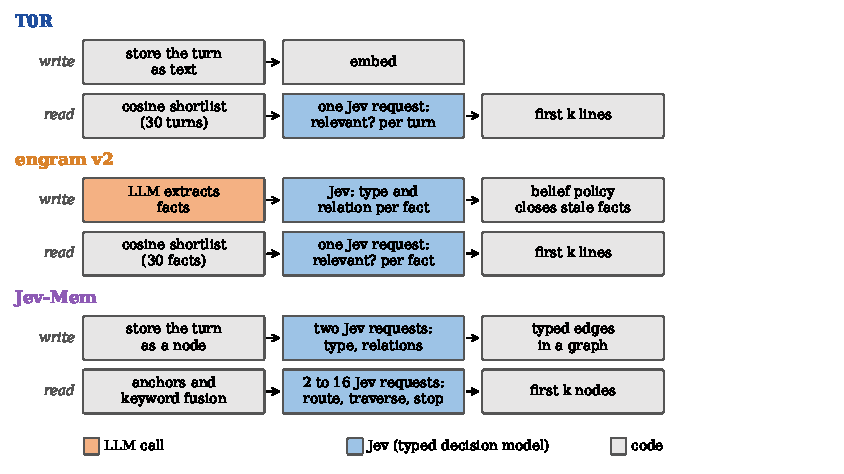
\includegraphics[width=\textwidth]{figures/paths.pdf}
\caption{Write and read paths of T0R, engram v2 and Jev-Mem. T0R writes raw turns with no LLM or Jev call and makes one Jev request per question; engram v2 extracts facts with an LLM and makes Jev decisions per fact at write time, then reads like T0R; Jev-Mem writes turns into a graph with two Jev requests each and makes several Jev requests per question.}\label{fig:1}
\end{figure*}
\textbf{T0R.} The write path embeds each turn and stores it as ``[date] speaker: text'', with no extraction and no LLM call. The read path takes a 30\src{docs/V3\_PLAN.md §1, §2, §4}-turn cosine shortlist and asks Jev, in one request, whether each turn helps answer the question; turns above 0.5\src{docs/V3\_PLAN.md §1, §2, §4} are kept in order of Jev's probability, followed by a cosine floor of 10\src{docs/V3\_PLAN.md §1, §2, §4} turns. The answer model sees the first k lines.

\textbf{L0.} The same store, read in cosine order with no Jev call.

\textbf{T0R-LLM.} T0R's store and shortlist, scored by a gpt-4o-mini listwise reranker instead of Jev.

\textbf{Full context.} Every turn of the conversation, rendered as T0R renders a line, in the answer prompt.

\textbf{engram v2.} An LLM extracts facts from each message with mem0's extraction prompt; Jev then answers typing questions and relation questions against up to ten candidate facts, and a belief policy closes superseded facts. The read path is T0R's over facts instead of turns. We use the frozen v2 system (tag \texttt{v2-frozen}).

\textbf{mem0 2.1.0.} The default \texttt{add()} path: one LLM extraction call per message, with the session date as the observation date; reads are vector search.

\textbf{Jev-Mem.} Jev-Mem at commit 81574eb with its default profile and \texttt{jev\_\allowbreak{}model} pinned to jev-1.13.0, driven through its own API. Each turn is a node; each write makes two Jev requests (memory type, relations), and each read routes, traverses and stops with between two and sixteen Jev requests. Its returned turns are rendered as ``[date] speaker: text'' and answered with our prompt; its own prompts, best-of-three selection and judge are not used.

\section{Study Design}\label{sec:4}
\textbf{Pre-registration.} The plan was deposited before any run on the data below (10.5281/zenodo.22970745, commit b3c5dc5, tag \texttt{v3-frozen}). An amendment, with the outcome paragraphs used in \cref{sec:5.1}, was deposited before any primary-test result was seen (10.5281/zenodo.22977848, commit efae0b6, tag \texttt{v3-amended}) \citep{sharma2026v3plan,sharma2026v3amend}.

\textbf{Data.} LoCoMo \citep{maharana2024locomo} numbers its question categories. We name them 1 multi-hop, 2 temporal, 3 open-domain, 4 single-hop and 5 adversarial, which matches the dataset's counts over all ten conversations (282\src{bench/data/locomo10.json (count of category 1, all ten conversations)}, 321\src{bench/data/locomo10.json (count of category 2, all ten conversations)}, 96\src{bench/data/locomo10.json (count of category 3, all ten conversations)}, 841\src{bench/data/locomo10.json (count of category 4, all ten conversations)} and 446\src{bench/data/locomo10.json (count of category 5, all ten conversations)} questions). The primary data are conv-44, conv-47, conv-48, conv-49 and conv-50, never run by any system before this study: 3,122\src{bench/results/v3/batch\_b\_report.json\#write/engram v2/turns} turns, 778\src{bench/results/v3/batch\_b\_report.json\#H1/questions} scored questions (140\src{bench/results/v3/lean\_t0r\_\_heldout\_*\_\_k3.json (count of category 1)} multi-hop, 165\src{bench/results/v3/lean\_t0r\_\_heldout\_*\_\_k3.json (count of category 2)} temporal, 50\src{bench/results/v3/lean\_t0r\_\_heldout\_*\_\_k3.json (count of category 3)} open-domain, 423\src{bench/results/v3/lean\_t0r\_\_heldout\_*\_\_k3.json (count of category 4)} single-hop) and 209\src{bench/results/v3/batch\_b\_report.json\#fresh\_adversarial/mem0 k3/questions} adversarial. conv-30, conv-41, conv-42 and conv-43 (610\src{bench/results/v3/batch\_a\_report.json\#exploratory/L0 k3/questions} scored questions), held out in an earlier study, give an exploratory replication. Development used conv-26 only. LongMemEval\_S cleaned \citep{wu2025longmemeval} provides a registered sample of 70\src{bench/results/v3/batch\_c\_report.json\#S6/questions} questions (user turns only) and, by amendment, all 500\src{bench/results/v3/batch\_c\_report.json (470 scored + 30 abstention)} questions with user and assistant turns (470\src{bench/results/v3/batch\_c\_report.json\#S7/questions} scored, 30\src{bench/results/v3/batch\_c\_report.json\#expansion/T0R 3 (abstention, correct = abstained)/questions} abstention).

\textbf{Stack.} Answers and judgments use gpt-4o-mini at temperature 0 with mem0's LoCoMo answer and judge prompts; the judge returns CORRECT or WRONG. Tokens are counted with o200k\_base over the memory block the answer model sees.

\textbf{Token matching.} Every comparison between systems holds context fixed. The comparator runs at $k{=}$3, its natural setting, and T0R is matched to it: from a retrieval-only sweep of T0R over k from one to thirty, the k whose pooled mean tokens per question is closest to the comparator's, ties going to the larger k. The sweep and the chosen k were saved before T0R answered at that k.

\textbf{Tests.} The primary test H1 asks whether T0R is non-inferior to engram v2: with d the per-question difference in correctness (T0R minus engram v2), non-inferiority holds if $\bar{d}$ $-$ 1.645$\cdot$SE exceeds $-$5\src{docs/V3\_PLAN.md §1, §2, §4} points. The margin is half the rerank's measured effect on the development conversation. The seven secondary tests, under Holm correction at family-wise 0.05, are exact two-sided McNemar tests except S4, a non-inferiority test with the same margin: S1 T0R against L0, S2 against Jev-Mem, S3 against mem0 and S4 against T0R-LLM on LoCoMo; S5 against mem0 and S6 against L0 on the LongMemEval sample; S7 against L0 on the full LongMemEval set. The plan's power analysis put the probability of passing H1 at 0.89\src{docs/V3\_PLAN.md §1, §2, §4} if the development difference held.

\textbf{Checks.} H1 and S1 were re-answered by Llama 3.3 70B Instruct via OpenRouter from the same contexts and judged by the same judge; a result is called model-robust only if it holds under both answer models. The author graded every question on which the judge found exactly one of H1's two answers correct, blind to system and judge label (\cref{sec:5.4}, \hyperref[app:C]{Appendix~C}). Shortlist recall measures where the LoCoMo evidence turns fall (\cref{sec:5.6}, \hyperref[app:D]{Appendix~D}).

\textbf{Deviations.} All are recorded in the plan with dates (\hyperref[app:B]{Appendix~B}): the amendment; mem0's extraction calls, which were served through OpenRouter (half of them by Azure) rather than the OpenAI API; runs repeated after rate limits; a token-counting fix for one LongMemEval haystack; the audit sheet's layout and grading standard; and the replacement of the title the registered outcome rule selected.

\section{Results}\label{sec:5}
\subsection{Primary test (H1, registered)}\label{sec:5.1}
\begin{table*}[tbp]
\centering
\footnotesize\hyphenpenalty=10000\exhyphenpenalty=10000\setlength{\tabcolsep}{4.5pt}
\caption{H1: T0R at $k{=}$6\src{bench/results/v3/batch\_b\_report.json\#token\_match/engram v2/t0r\_k} (265\src{bench/results/v3/batch\_b\_report.json\#fresh/T0R k6 (matched to engram v2)/tokens\_mean} tokens per question) against engram v2 at $k{=}$3 (251\src{bench/results/v3/batch\_b\_report.json\#token\_match/engram v2/comparator\_k3} tokens), 778\src{bench/results/v3/batch\_b\_report.json\#H1/questions} scored questions of the five held-out conversations. The judge row is the registered test; the human rows replace the judge's labels on the 141\src{bench/results/v3/human\_audit/audit\_report.json\#strict/discordant\_questions\_graded} graded discordant questions. Differences and bounds in points.}\label{tab:1}
\begin{tabular}{@{}>{\raggedright\arraybackslash}p{97.4pt}>{\raggedleft\arraybackslash}p{30.7pt}>{\raggedleft\arraybackslash}p{37.2pt}>{\raggedleft\arraybackslash}p{52.7pt}>{\raggedleft\arraybackslash}p{46.7pt}>{\raggedleft\arraybackslash}p{55.1pt}>{\raggedright\arraybackslash}p{81.1pt}@{}}
\toprule
\textbf{Grading} & \textbf{T0R} & \textbf{engram v2} & \textbf{Difference} & \textbf{One-sided 95\% bound} & \textbf{Two-sided 95\% CI} & \textbf{Non-inferior (margin $-$5\src{docs/V3\_PLAN.md §1, §2, §4})} \\
\midrule
Judge (registered) & 77.0\%\src{bench/results/v3/batch\_b\_report.json\#H1/acc\_a} & 77.5\%\src{bench/results/v3/batch\_b\_report.json\#H1/acc\_b} & $-$0.5\src{bench/results/v3/batch\_b\_report.json\#H1/d\_bar} & $-$3.0\src{bench/results/v3/batch\_b\_report.json\#H1/lower\_bound\_95\_one\_sided} & [$-$3.5\src{bench/results/v3/batch\_b\_report.json\#H1 (d\_bar - 1.96 se)},~+2.5\src{bench/results/v3/batch\_b\_report.json\#H1 (d\_bar + 1.96 se)}] & yes \\
Human, strict & 76.3\%\src{bench/results/v3/human\_audit/audit\_report.json\#strict/H1\_with\_human\_grades/acc\_t0r} & 78.0\%\src{bench/results/v3/human\_audit/audit\_report.json\#strict/H1\_with\_human\_grades/acc\_engram} & $-$1.7\src{bench/results/v3/human\_audit/audit\_report.json\#strict/H1\_with\_human\_grades/d\_bar} & $-$3.9\src{bench/results/v3/human\_audit/audit\_report.json\#strict/H1\_with\_human\_grades/lower\_bound\_95\_one\_sided} & [$-$4.3\src{bench/results/v3/human\_audit/audit\_report.json\#strict/H1\_with\_human\_grades/ci95\_two\_sided/0},~+0.9\src{bench/results/v3/human\_audit/audit\_report.json\#strict/H1\_with\_human\_grades/ci95\_two\_sided/1}] & yes \\
Human, lenient & 77.4\%\src{bench/results/v3/human\_audit/audit\_report.json\#lenient/H1\_with\_human\_grades/acc\_t0r} & 79.9\%\src{bench/results/v3/human\_audit/audit\_report.json\#lenient/H1\_with\_human\_grades/acc\_engram} & $-$2.6\src{bench/results/v3/human\_audit/audit\_report.json\#lenient/H1\_with\_human\_grades/d\_bar} & $-$4.7\src{bench/results/v3/human\_audit/audit\_report.json\#lenient/H1\_with\_human\_grades/lower\_bound\_95\_one\_sided} & [$-$5.1\src{bench/results/v3/human\_audit/audit\_report.json\#lenient/H1\_with\_human\_grades/ci95\_two\_sided/0},~$-$0.03\src{bench/results/v3/human\_audit/audit\_report.json\#lenient/H1\_with\_human\_grades/ci95\_two\_sided/1}] & yes \\
\bottomrule
\end{tabular}
\end{table*}
The registered outcome paragraph, filled in:

\begin{quote}
Pass. At matched context (265\src{bench/results/v3/batch\_b\_report.json\#fresh/T0R k6 (matched to engram v2)/tokens\_mean} tokens; engram v2 251\src{bench/results/v3/batch\_b\_report.json\#token\_match/engram v2/comparator\_k3}), raw turns with a single rerank call were non-inferior to LLM-extraction memory: difference $-$0.5\src{bench/results/v3/batch\_b\_report.json\#H1/d\_bar} points, one-sided 95\% lower bound $-$3.0\src{bench/results/v3/batch\_b\_report.json\#H1/lower\_bound\_95\_one\_sided}, above the registered $-$5\src{docs/V3\_PLAN.md §1, §2, §4} margin. Whatever accuracy extraction adds at this budget is under 3.0\src{bench/results/v3/batch\_b\_report.json\#H1/lower\_bound\_95\_one\_sided (negated)} points, at 3,061\src{bench/results/v3/batch\_b\_report.json\#write\_cost\_ratio\_engram\_over\_t0r/ratio}$\times$ the write cost. The rerank closes 94\%\src{bench/results/v3/batch\_b\_report.json\#G/G} of the gap between similarity search and extraction. By category, T0R did not trail on multi-hop (74.3\src{bench/results/v3/batch\_b\_report.json\#fresh/T0R k6 (matched to engram v2)/by\_category/multi-hop} vs 72.1\src{bench/results/v3/batch\_b\_report.json\#fresh/engram v2 k3/by\_category/multi-hop}, n=140\src{bench/results/v3/lean\_t0r\_\_heldout\_*\_\_k3.json (count of category 1)}) and trailed on open-domain (56.0\src{bench/results/v3/batch\_b\_report.json\#fresh/T0R k6 (matched to engram v2)/by\_category/open-domain} vs 60.0\src{bench/results/v3/batch\_b\_report.json\#fresh/engram v2 k3/by\_category/open-domain}, n=50\src{bench/results/v3/lean\_t0r\_\_heldout\_*\_\_k3.json (count of category 3)}), contrary to what we registered for multi-hop and as we registered for open-domain.
\end{quote}

The one-sided p-value is 0.0017\src{bench/results/v3/batch\_b\_report.json\#H1/p\_one\_sided}, and the conversation bootstrap puts the fifth percentile of the difference at $-$2.3\src{bench/results/v3/batch\_b\_report.json\#H1/bootstrap\_conversations\_5th\_percentile} points. 69\src{bench/results/v3/batch\_b\_report.json\#H1/only\_a} questions were answered correctly only by T0R and 73\src{bench/results/v3/batch\_b\_report.json\#H1/only\_b} only by engram v2. Human grading moves the difference to between $-$1.7\src{bench/results/v3/human\_audit/audit\_report.json\#strict/H1\_with\_human\_grades/d\_bar} and $-$2.6\src{bench/results/v3/human\_audit/audit\_report.json\#lenient/H1\_with\_human\_grades/d\_bar} points and the bound to between $-$3.9\src{bench/results/v3/human\_audit/audit\_report.json\#strict/H1\_with\_human\_grades/lower\_bound\_95\_one\_sided} and $-$4.7\src{bench/results/v3/human\_audit/audit\_report.json\#lenient/H1\_with\_human\_grades/lower\_bound\_95\_one\_sided}; under lenient grading the two-sided interval lies just below zero, so by that grading engram v2 is more accurate, still inside the margin. We therefore state the result as: non-inferior within a 5\src{docs/V3\_PLAN.md §1, §2, §4}-point margin under every grading we applied, with extraction adding at most 4.7\src{bench/results/v3/human\_audit/audit\_report.json\#lenient/H1\_with\_human\_grades/lower\_bound\_95\_one\_sided (negated)} points at this budget. The category comparisons are descriptive; the categories are small and the differences are not tested.

G, the share of the gap between similarity search and extraction that the rerank closes, uses L0 at its own matched k (6\src{bench/results/v3/batch\_b\_report.json\#G/l0\_k}, 68.6\%\src{bench/results/v3/batch\_b\_report.json\#G/l0} accuracy): at the same token budget, one rerank call closes G = 94\%\src{bench/results/v3/batch\_b\_report.json\#G/G} of the accuracy gap between cosine retrieval of raw turns (L0, 68.6\%\src{bench/results/v3/batch\_b\_report.json\#G/l0}) and LLM-extracted memory (engram v2, 77.5\%\src{bench/results/v3/batch\_b\_report.json\#H1/acc\_b}). The write-cost ratio uses held-out measurements: engram v2 costs \$1.865\src{bench/results/v3/batch\_b\_report.json\#write\_cost\_ratio\_engram\_over\_t0r/engram\_v2\_per\_1k} per 1,000 turns and T0R \$0.00061\src{bench/results/v3/batch\_b\_report.json\#write\_cost\_ratio\_engram\_over\_t0r/t0r\_per\_1k} (embeddings only), at list prices.

\subsection{Secondary tests (S1--S7, registered)}\label{sec:5.2}
\begin{table*}[tbp]
\centering
\footnotesize\hyphenpenalty=10000\exhyphenpenalty=10000\setlength{\tabcolsep}{4.5pt}
\caption{Secondary tests. In each, the comparator runs at $k{=}$3 and T0R at its matched k. ``Only T0R'' and ``only other'' count questions answered correctly by one system. S4 is a non-inferiority test (one-sided p); the rest are exact two-sided McNemar tests. Holm adjustment over S1--S7. LoCoMo tests use 778\src{bench/results/v3/batch\_b\_report.json\#H1/questions} questions; LongMemEval ingestion: user turns for S5--S6, user and assistant turns for S7.}\label{tab:2}
\begin{tabular}{@{}>{\raggedright\arraybackslash}p{27.2pt}>{\raggedright\arraybackslash}p{197.0pt}>{\raggedleft\arraybackslash}p{20.1pt}>{\raggedleft\arraybackslash}p{25.9pt}>{\raggedleft\arraybackslash}p{25.9pt}>{\raggedleft\arraybackslash}p{32.1pt}>{\raggedleft\arraybackslash}p{31.9pt}>{\raggedleft\arraybackslash}p{31.9pt}@{}}
\toprule
\textbf{Test} & \textbf{Comparison} & \textbf{T0R k} & \textbf{T0R} & \textbf{Other} & \textbf{Only T0R / only other} & \textbf{p} & \textbf{Holm p} \\
\midrule
S1 & T0R vs L0 (LoCoMo) & 3\src{bench/results/v3/batch\_a\_report.json\#token\_match/L0/t0r\_k} & 77.2\%\src{bench/results/v3/batch\_a\_report.json\#S1/acc\_a} & 59.9\%\src{bench/results/v3/batch\_a\_report.json\#S1/acc\_b} & 152\src{bench/results/v3/batch\_a\_report.json\#S1/only\_a} / 17\src{bench/results/v3/batch\_a\_report.json\#S1/only\_b} & 2.7e$-$28\src{bench/results/v3/batch\_a\_report.json\#S1/p\_two\_sided} & 1.9e$-$27\src{bench/results/v3/batch\_c\_report.json\#holm\_S1\_S7/S1/holm\_adjusted\_p} \\
S2 & T0R vs Jev-Mem (LoCoMo) & 4\src{bench/results/v3/batch\_a\_report.json\#token\_match/Jev-Mem/t0r\_k} & 77.0\%\src{bench/results/v3/batch\_a\_report.json\#S2/acc\_a} & 70.6\%\src{bench/results/v3/batch\_a\_report.json\#S2/acc\_b} & 98\src{bench/results/v3/batch\_a\_report.json\#S2/only\_a} / 48\src{bench/results/v3/batch\_a\_report.json\#S2/only\_b} & 4.3e$-$5\src{bench/results/v3/batch\_a\_report.json\#S2/p\_two\_sided} & 1.3e$-$4\src{bench/results/v3/batch\_c\_report.json\#holm\_S1\_S7/S2/holm\_adjusted\_p} \\
S3 & T0R vs mem0 (LoCoMo) & 3\src{bench/results/v3/batch\_b\_report.json\#token\_match/mem0/t0r\_k} & 77.2\%\src{bench/results/v3/batch\_b\_report.json\#S3/acc\_a} & 68.5\%\src{bench/results/v3/batch\_b\_report.json\#S3/acc\_b} & 134\src{bench/results/v3/batch\_b\_report.json\#S3/only\_a} / 66\src{bench/results/v3/batch\_b\_report.json\#S3/only\_b} & 1.7e$-$6\src{bench/results/v3/batch\_b\_report.json\#S3/p\_two\_sided} & 7.6e$-$6\src{bench/results/v3/batch\_c\_report.json\#holm\_S1\_S7/S3/holm\_adjusted\_p} \\
S4 & T0R vs T0R-LLM (LoCoMo, non-inferiority) & 3\src{bench/results/v3/batch\_b\_report.json\#token\_match/T0R-LLM/t0r\_k} & 77.2\%\src{bench/results/v3/batch\_b\_report.json\#S4/acc\_a} & 77.6\%\src{bench/results/v3/batch\_b\_report.json\#S4/acc\_b} & 28\src{bench/results/v3/batch\_b\_report.json\#S4/only\_a} / 31\src{bench/results/v3/batch\_b\_report.json\#S4/only\_b} & 1.5e$-$6\src{bench/results/v3/batch\_b\_report.json\#S4/p\_one\_sided} & 7.6e$-$6\src{bench/results/v3/batch\_c\_report.json\#holm\_S1\_S7/S4/holm\_adjusted\_p} \\
S5 & T0R vs mem0 (LongMemEval, 30\src{bench/results/v3/batch\_c\_report.json\#S5/questions} knowledge-update) & 2\src{bench/results/v3/batch\_c\_report.json\#token\_match/sample: T0R vs mem0 3/t0r\_k} & 70.0\%\src{bench/results/v3/batch\_c\_report.json\#S5/acc\_a} & 70.0\%\src{bench/results/v3/batch\_c\_report.json\#S5/acc\_b} & 4\src{bench/results/v3/batch\_c\_report.json\#S5/only\_a} / 4\src{bench/results/v3/batch\_c\_report.json\#S5/only\_b} & 1.00\src{bench/results/v3/batch\_c\_report.json\#S5/p\_two\_sided} & 1.00\src{bench/results/v3/batch\_c\_report.json\#holm\_S1\_S7/S5/holm\_adjusted\_p} \\
S6 & T0R vs L0 (LongMemEval sample, 70\src{bench/results/v3/batch\_c\_report.json\#S6/questions}) & 3\src{bench/results/v3/batch\_c\_report.json\#token\_match/sample: T0R vs L0 3/t0r\_k} & 68.6\%\src{bench/results/v3/batch\_c\_report.json\#S6/acc\_a} & 65.7\%\src{bench/results/v3/batch\_c\_report.json\#S6/acc\_b} & 7\src{bench/results/v3/batch\_c\_report.json\#S6/only\_a} / 5\src{bench/results/v3/batch\_c\_report.json\#S6/only\_b} & 0.77\src{bench/results/v3/batch\_c\_report.json\#S6/p\_two\_sided} & 1.00\src{bench/results/v3/batch\_c\_report.json\#holm\_S1\_S7/S6/holm\_adjusted\_p} \\
S7 & T0R vs L0 (LongMemEval, 470\src{bench/results/v3/batch\_c\_report.json\#S7/questions}) & 3\src{bench/results/v3/batch\_c\_report.json\#token\_match/expansion: T0R vs L0 3/t0r\_k} & 66.8\%\src{bench/results/v3/batch\_c\_report.json\#S7/acc\_a} & 57.7\%\src{bench/results/v3/batch\_c\_report.json\#S7/acc\_b} & 61\src{bench/results/v3/batch\_c\_report.json\#S7/only\_a} / 18\src{bench/results/v3/batch\_c\_report.json\#S7/only\_b} & 1.3e$-$6\src{bench/results/v3/batch\_c\_report.json\#S7/p\_two\_sided} & 7.6e$-$6\src{bench/results/v3/batch\_c\_report.json\#holm\_S1\_S7/S7/holm\_adjusted\_p} \\
\bottomrule
\end{tabular}
\end{table*}
S1, S2, S3, S4 and S7 are rejected after Holm correction; S5 and S6 are not. On LoCoMo, T0R was more accurate than similarity search (S1), Jev-Mem (S2) and mem0 (S3) at matched context, and non-inferior to the LLM reranker (S4: difference $-$0.4\src{bench/results/v3/batch\_b\_report.json\#S4/d\_bar} points, lower bound $-$2.0\src{bench/results/v3/batch\_b\_report.json\#S4/lower\_bound\_95\_one\_sided}). S3 carries a caveat: mem0's extraction was served through OpenRouter, about half of it by Azure (\hyperref[app:G]{Appendix~G}). On the LongMemEval sample, S5 detected no difference between T0R and mem0 on 30\src{bench/results/v3/batch\_c\_report.json\#S5/questions} knowledge-update questions, which is too few to establish equivalence, and S6 detected none between T0R and L0 on 70\src{bench/results/v3/batch\_c\_report.json\#S6/questions} questions. On the full set, S7 found T0R more accurate than L0 by +9.1\src{bench/results/v3/batch\_c\_report.json\#S7 (acc\_a - acc\_b)} points. By the registered rule, LongMemEval holds: S7 favours T0R after Holm correction and S5 does not favour mem0.

\subsection{The budget dependence of reranking}\label{sec:5.3}
The rerank's value depends on how many candidates the budget keeps (Figures~\ref{fig:2} and \ref{fig:3}). On LoCoMo its gain over similarity search is +17.4\src{bench/results/v3/batch\_a\_report.json\#fresh (T0R k3 - L0 k3)} points at $k{=}$3 and +1.5\src{bench/results/v3/batch\_a\_report.json\#fresh (T0R k20 - L0 k20)} at $k{=}$20. On the full LongMemEval set it is +9.1\src{bench/results/v3/batch\_c\_report.json\#expansion (T0R 3 - L0 3)} points at $k{=}$3 (S7) and +1.1\src{bench/results/v3/batch\_c\_report.json\#expansion (T0R 20 - L0 20)} at $k{=}$20. With three of 30\src{docs/V3\_PLAN.md §1, §2, §4} candidates kept, ordering decides which evidence reaches the answer model; with twenty kept, cosine order already includes most of it. The $k{=}$3 gains are registered tests (S1, S7); the $k{=}$20 differences are descriptive.

\begin{figure}[tbp]
\centering
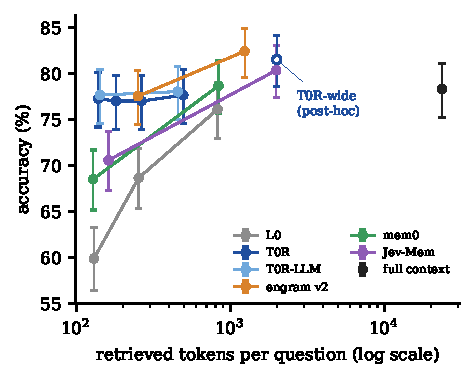
\includegraphics[width=\columnwidth]{figures/budget_locomo.pdf}
\caption{LoCoMo accuracy against retrieved tokens per question (log scale), five held-out conversations, 778 questions, Wilson 95\% intervals. T0R at every measured k; T0R-wide is post-hoc (hollow marker).}\label{fig:2}
\end{figure}
\begin{figure}[tbp]
\centering
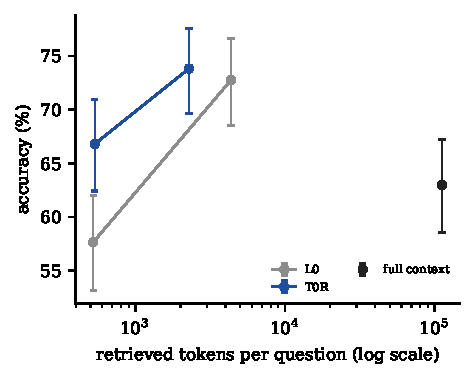
\includegraphics[width=\columnwidth]{figures/budget_lme.pdf}
\caption{LongMemEval accuracy against retrieved tokens per question (log scale), 470 non-abstention questions, user and assistant turns, Wilson 95\% intervals.}\label{fig:3}
\end{figure}
T0R at $k{=}$3 is within 1.0\src{bench/results/v3/batch\_b\_report.json\#fresh (full context - T0R k3)} points of full context on LoCoMo while reading 139\src{bench/results/v3/batch\_a\_report.json\#fresh/T0R k3/tokens\_mean} tokens per question instead of 23,631\src{bench/results/v3/batch\_b\_report.json\#fresh/full context all turns/tokens\_mean}. At generous budgets the ordering reverses (Table~\ref{tab:3}): engram v2 at $k{=}$20 reaches 82.4\%\src{bench/results/v3/batch\_b\_report.json\#fresh/engram v2 k20/accuracy}, Jev-Mem at $k{=}$40 80.3\%\src{bench/results/v3/batch\_a\_report.json\#fresh/Jev-Mem k40/accuracy}, mem0 at $k{=}$20 78.7\%\src{bench/results/v3/batch\_b\_report.json\#fresh/mem0 k20/accuracy} and full context 78.3\%\src{bench/results/v3/batch\_b\_report.json\#fresh/full context all turns/accuracy}, while T0R stays near 77.6\%\src{bench/results/v3/batch\_a\_report.json\#fresh/T0R k20/accuracy} at any k (\cref{sec:5.6}).

\begin{table*}[tbp]
\centering
\footnotesize\hyphenpenalty=10000\exhyphenpenalty=10000\setlength{\tabcolsep}{4.5pt}
\caption{LoCoMo, five held-out conversations, 778\src{bench/results/v3/batch\_b\_report.json\#H1/questions} scored questions: accuracy (\%), tokens per question and accuracy by category.}\label{tab:3}
\begin{tabular}{@{}>{\raggedright\arraybackslash}p{118.0pt}>{\raggedleft\arraybackslash}p{46.1pt}>{\raggedleft\arraybackslash}p{37.1pt}>{\raggedleft\arraybackslash}p{43.7pt}>{\raggedleft\arraybackslash}p{47.0pt}>{\raggedleft\arraybackslash}p{59.0pt}>{\raggedleft\arraybackslash}p{50.0pt}@{}}
\toprule
\textbf{System, setting} & \textbf{Accuracy} & \textbf{Tokens} & \textbf{Multi-hop} & \textbf{Temporal} & \textbf{Open-domain} & \textbf{Single-hop} \\
\midrule
L0, $k{=}$3 & 59.9\%\src{bench/results/v3/batch\_a\_report.json\#fresh/L0 k3/accuracy} & 130\src{bench/results/v3/batch\_a\_report.json\#fresh/L0 k3/tokens\_mean} & 54.3\src{bench/results/v3/batch\_a\_report.json\#fresh/L0 k3/by\_category/multi-hop} & 55.2\src{bench/results/v3/batch\_a\_report.json\#fresh/L0 k3/by\_category/temporal} & 42.0\src{bench/results/v3/batch\_a\_report.json\#fresh/L0 k3/by\_category/open-domain} & 65.7\src{bench/results/v3/batch\_a\_report.json\#fresh/L0 k3/by\_category/single-hop} \\
L0, $k{=}$6 & 68.6\%\src{bench/results/v3/batch\_b\_report.json\#fresh/L0 k6 (matched to engram v2, for G)/accuracy} & 254\src{bench/results/v3/batch\_b\_report.json\#fresh/L0 k6 (matched to engram v2, for G)/tokens\_mean} & 61.4\src{bench/results/v3/batch\_b\_report.json\#fresh/L0 k6 (matched to engram v2, for G)/by\_category/multi-hop} & 60.6\src{bench/results/v3/batch\_b\_report.json\#fresh/L0 k6 (matched to engram v2, for G)/by\_category/temporal} & 54.0\src{bench/results/v3/batch\_b\_report.json\#fresh/L0 k6 (matched to engram v2, for G)/by\_category/open-domain} & 75.9\src{bench/results/v3/batch\_b\_report.json\#fresh/L0 k6 (matched to engram v2, for G)/by\_category/single-hop} \\
L0, $k{=}$20 & 76.1\%\src{bench/results/v3/batch\_a\_report.json\#fresh/L0 k20/accuracy} & 826\src{bench/results/v3/batch\_a\_report.json\#fresh/L0 k20/tokens\_mean} & 68.6\src{bench/results/v3/batch\_a\_report.json\#fresh/L0 k20/by\_category/multi-hop} & 68.5\src{bench/results/v3/batch\_a\_report.json\#fresh/L0 k20/by\_category/temporal} & 58.0\src{bench/results/v3/batch\_a\_report.json\#fresh/L0 k20/by\_category/open-domain} & 83.7\src{bench/results/v3/batch\_a\_report.json\#fresh/L0 k20/by\_category/single-hop} \\
T0R, $k{=}$3 & 77.2\%\src{bench/results/v3/batch\_a\_report.json\#fresh/T0R k3/accuracy} & 139\src{bench/results/v3/batch\_a\_report.json\#fresh/T0R k3/tokens\_mean} & 75.7\src{bench/results/v3/batch\_a\_report.json\#fresh/T0R k3/by\_category/multi-hop} & 69.1\src{bench/results/v3/batch\_a\_report.json\#fresh/T0R k3/by\_category/temporal} & 58.0\src{bench/results/v3/batch\_a\_report.json\#fresh/T0R k3/by\_category/open-domain} & 83.2\src{bench/results/v3/batch\_a\_report.json\#fresh/T0R k3/by\_category/single-hop} \\
T0R, $k{=}$6 & 77.0\%\src{bench/results/v3/batch\_b\_report.json\#fresh/T0R k6 (matched to engram v2)/accuracy} & 265\src{bench/results/v3/batch\_b\_report.json\#fresh/T0R k6 (matched to engram v2)/tokens\_mean} & 74.3\src{bench/results/v3/batch\_b\_report.json\#fresh/T0R k6 (matched to engram v2)/by\_category/multi-hop} & 72.1\src{bench/results/v3/batch\_b\_report.json\#fresh/T0R k6 (matched to engram v2)/by\_category/temporal} & 56.0\src{bench/results/v3/batch\_b\_report.json\#fresh/T0R k6 (matched to engram v2)/by\_category/open-domain} & 82.3\src{bench/results/v3/batch\_b\_report.json\#fresh/T0R k6 (matched to engram v2)/by\_category/single-hop} \\
T0R, $k{=}$20 & 77.6\%\src{bench/results/v3/batch\_a\_report.json\#fresh/T0R k20/accuracy} & 496\src{bench/results/v3/batch\_a\_report.json\#fresh/T0R k20/tokens\_mean} & 75.0\src{bench/results/v3/batch\_a\_report.json\#fresh/T0R k20/by\_category/multi-hop} & 72.7\src{bench/results/v3/batch\_a\_report.json\#fresh/T0R k20/by\_category/temporal} & 58.0\src{bench/results/v3/batch\_a\_report.json\#fresh/T0R k20/by\_category/open-domain} & 82.7\src{bench/results/v3/batch\_a\_report.json\#fresh/T0R k20/by\_category/single-hop} \\
T0R-LLM, $k{=}$3 & 77.6\%\src{bench/results/v3/batch\_b\_report.json\#fresh/T0R-LLM k3/accuracy} & 143\src{bench/results/v3/batch\_b\_report.json\#fresh/T0R-LLM k3/tokens\_mean} & 73.6\src{bench/results/v3/batch\_b\_report.json\#fresh/T0R-LLM k3/by\_category/multi-hop} & 72.7\src{bench/results/v3/batch\_b\_report.json\#fresh/T0R-LLM k3/by\_category/temporal} & 58.0\src{bench/results/v3/batch\_b\_report.json\#fresh/T0R-LLM k3/by\_category/open-domain} & 83.2\src{bench/results/v3/batch\_b\_report.json\#fresh/T0R-LLM k3/by\_category/single-hop} \\
T0R-LLM, $k{=}$20 & 78.0\%\src{bench/results/v3/batch\_b\_report.json\#fresh/T0R-LLM k20/accuracy} & 456\src{bench/results/v3/batch\_b\_report.json\#fresh/T0R-LLM k20/tokens\_mean} & 72.9\src{bench/results/v3/batch\_b\_report.json\#fresh/T0R-LLM k20/by\_category/multi-hop} & 71.5\src{bench/results/v3/batch\_b\_report.json\#fresh/T0R-LLM k20/by\_category/temporal} & 60.0\src{bench/results/v3/batch\_b\_report.json\#fresh/T0R-LLM k20/by\_category/open-domain} & 84.4\src{bench/results/v3/batch\_b\_report.json\#fresh/T0R-LLM k20/by\_category/single-hop} \\
engram v2, $k{=}$3 & 77.5\%\src{bench/results/v3/batch\_b\_report.json\#fresh/engram v2 k3/accuracy} & 251\src{bench/results/v3/batch\_b\_report.json\#fresh/engram v2 k3/tokens\_mean} & 72.1\src{bench/results/v3/batch\_b\_report.json\#fresh/engram v2 k3/by\_category/multi-hop} & 77.6\src{bench/results/v3/batch\_b\_report.json\#fresh/engram v2 k3/by\_category/temporal} & 60.0\src{bench/results/v3/batch\_b\_report.json\#fresh/engram v2 k3/by\_category/open-domain} & 81.3\src{bench/results/v3/batch\_b\_report.json\#fresh/engram v2 k3/by\_category/single-hop} \\
engram v2, $k{=}$20 & 82.4\%\src{bench/results/v3/batch\_b\_report.json\#fresh/engram v2 k20/accuracy} & 1,238\src{bench/results/v3/batch\_b\_report.json\#fresh/engram v2 k20/tokens\_mean} & 77.9\src{bench/results/v3/batch\_b\_report.json\#fresh/engram v2 k20/by\_category/multi-hop} & 80.0\src{bench/results/v3/batch\_b\_report.json\#fresh/engram v2 k20/by\_category/temporal} & 64.0\src{bench/results/v3/batch\_b\_report.json\#fresh/engram v2 k20/by\_category/open-domain} & 87.0\src{bench/results/v3/batch\_b\_report.json\#fresh/engram v2 k20/by\_category/single-hop} \\
mem0, $k{=}$3 & 68.5\%\src{bench/results/v3/batch\_b\_report.json\#fresh/mem0 k3/accuracy} & 129\src{bench/results/v3/batch\_b\_report.json\#fresh/mem0 k3/tokens\_mean} & 56.4\src{bench/results/v3/batch\_b\_report.json\#fresh/mem0 k3/by\_category/multi-hop} & 67.3\src{bench/results/v3/batch\_b\_report.json\#fresh/mem0 k3/by\_category/temporal} & 56.0\src{bench/results/v3/batch\_b\_report.json\#fresh/mem0 k3/by\_category/open-domain} & 74.5\src{bench/results/v3/batch\_b\_report.json\#fresh/mem0 k3/by\_category/single-hop} \\
mem0, $k{=}$20 & 78.7\%\src{bench/results/v3/batch\_b\_report.json\#fresh/mem0 k20/accuracy} & 839\src{bench/results/v3/batch\_b\_report.json\#fresh/mem0 k20/tokens\_mean} & 74.3\src{bench/results/v3/batch\_b\_report.json\#fresh/mem0 k20/by\_category/multi-hop} & 76.4\src{bench/results/v3/batch\_b\_report.json\#fresh/mem0 k20/by\_category/temporal} & 54.0\src{bench/results/v3/batch\_b\_report.json\#fresh/mem0 k20/by\_category/open-domain} & 83.9\src{bench/results/v3/batch\_b\_report.json\#fresh/mem0 k20/by\_category/single-hop} \\
Jev-Mem, $k{=}$3 & 70.6\%\src{bench/results/v3/batch\_a\_report.json\#fresh/Jev-Mem k3/accuracy} & 162\src{bench/results/v3/batch\_a\_report.json\#fresh/Jev-Mem k3/tokens\_mean} & 57.9\src{bench/results/v3/batch\_a\_report.json\#fresh/Jev-Mem k3/by\_category/multi-hop} & 64.2\src{bench/results/v3/batch\_a\_report.json\#fresh/Jev-Mem k3/by\_category/temporal} & 50.0\src{bench/results/v3/batch\_a\_report.json\#fresh/Jev-Mem k3/by\_category/open-domain} & 79.7\src{bench/results/v3/batch\_a\_report.json\#fresh/Jev-Mem k3/by\_category/single-hop} \\
Jev-Mem, $k{=}$40 & 80.3\%\src{bench/results/v3/batch\_a\_report.json\#fresh/Jev-Mem k40/accuracy} & 1,987\src{bench/results/v3/batch\_a\_report.json\#fresh/Jev-Mem k40/tokens\_mean} & 76.4\src{bench/results/v3/batch\_a\_report.json\#fresh/Jev-Mem k40/by\_category/multi-hop} & 73.9\src{bench/results/v3/batch\_a\_report.json\#fresh/Jev-Mem k40/by\_category/temporal} & 54.0\src{bench/results/v3/batch\_a\_report.json\#fresh/Jev-Mem k40/by\_category/open-domain} & 87.2\src{bench/results/v3/batch\_a\_report.json\#fresh/Jev-Mem k40/by\_category/single-hop} \\
Full context & 78.3\%\src{bench/results/v3/batch\_b\_report.json\#fresh/full context all turns/accuracy} & 23,631\src{bench/results/v3/batch\_b\_report.json\#fresh/full context all turns/tokens\_mean} & 78.6\src{bench/results/v3/batch\_b\_report.json\#fresh/full context all turns/by\_category/multi-hop} & 57.0\src{bench/results/v3/batch\_b\_report.json\#fresh/full context all turns/by\_category/temporal} & 64.0\src{bench/results/v3/batch\_b\_report.json\#fresh/full context all turns/by\_category/open-domain} & 88.2\src{bench/results/v3/batch\_b\_report.json\#fresh/full context all turns/by\_category/single-hop} \\
\bottomrule
\end{tabular}
\end{table*}
\subsection{Robustness: a second answer model and blind human grading}\label{sec:5.4}
With Llama 3.3 70B Instruct answering from the same contexts, H1 still passes (T0R 75.3\%\src{bench/results/v3/second\_model\_report.json\#H1/llama-3.3-70b/acc\_a}, engram v2 75.6\%\src{bench/results/v3/second\_model\_report.json\#H1/llama-3.3-70b/acc\_b}, difference $-$0.3\src{bench/results/v3/second\_model\_report.json\#H1/llama-3.3-70b/d\_bar}, one-sided bound $-$2.9\src{bench/results/v3/second\_model\_report.json\#H1/llama-3.3-70b/lower\_bound\_95\_one\_sided}) and so does S1 (T0R 74.9\%\src{bench/results/v3/second\_model\_report.json\#S1/llama-3.3-70b/acc\_a}, L0 57.6\%\src{bench/results/v3/second\_model\_report.json\#S1/llama-3.3-70b/acc\_b}, p = 5.8e$-$26\src{bench/results/v3/second\_model\_report.json\#S1/llama-3.3-70b/p\_two\_sided}). Both are therefore model-robust by the registered rule. Of 3,112\src{bench/results/v3/second\_model\_report.json (four arms x 778 questions)} rebuilt contexts, all but 4\src{bench/results/v3/second\_model\_report.json\#context\_mismatches} matched their recorded token counts exactly; the four come from near-tie reorderings. OpenRouter served Llama through 9\src{bench/results/v3/second\_model\_report.json\#providers (count)} providers whose numeric precision may differ.

The author graded, blind, both answers to each of H1's 142\src{bench/results/v3/batch\_b\_report.json\#H1 (only\_a + only\_b)} judge-discordant questions (284\src{bench/results/v3/human\_audit/audit\_report.json\#rows} rows; one question was left ungraded). Agreement with the judge was 81\%\src{bench/results/v3/human\_audit/audit\_report.json\#strict/agreement\_with\_judge} under the strict mapping and 79\%\src{bench/results/v3/human\_audit/audit\_report.json\#lenient/agreement\_with\_judge} under the lenient one (\hyperref[app:C]{Appendix~C}). Many judge-discordant pairs were not discordant to the human grader: under the strict mapping both answers were correct for 17\src{bench/results/v3/human\_audit/audit\_report.json\#strict/human\_both\_correct} questions and both wrong for 18\src{bench/results/v3/human\_audit/audit\_report.json\#strict/human\_both\_wrong}. The judge credited T0R's short answers more readily and engram v2's list-style answers less (agreement on engram v2's answers 77\%\src{bench/results/v3/human\_audit/audit\_report.json\#lenient/agreement\_with\_judge\_by\_system/engram} under the lenient mapping, against 82\%\src{bench/results/v3/human\_audit/audit\_report.json\#lenient/agreement\_with\_judge\_by\_system/T0R} on T0R's), which is why human grading widens the gap.

\subsection{Long histories (LongMemEval)}\label{sec:5.5}
LongMemEval compares T0R with mem0 and L0 only; engram v2 was not run on it, so these results cannot support any claim that T0R matches LLM-extracted memory on long histories. What they support is narrower: on histories of about 111,770\src{bench/results/v3/batch\_c\_report.json\#expansion/full context (non-abstention)/tokens\_mean} rendered tokens, the rerank still beats similarity search (S7), and no difference from mem0 was detected on knowledge-update questions (S5).

\begin{table*}[tbp]
\centering
\footnotesize\hyphenpenalty=10000\exhyphenpenalty=10000\setlength{\tabcolsep}{3.5pt}
\caption{LongMemEval, all 500\src{bench/results/v3/batch\_c\_report.json (470 scored + 30 abstention)} questions, user and assistant turns ingested: accuracy (\%) on the 470\src{bench/results/v3/batch\_c\_report.json\#S7/questions} non-abstention questions, by question type (n), and the share of the 30\src{bench/results/v3/batch\_c\_report.json\#expansion/T0R 3 (abstention, correct = abstained)/questions} abstention questions answered by abstaining.}\label{tab:4}
\begin{tabular}{@{}>{\raggedright\arraybackslash}p{36.1pt}>{\raggedleft\arraybackslash}p{32.6pt}>{\raggedleft\arraybackslash}p{25.3pt}>{\raggedleft\arraybackslash}p{37.1pt}>{\raggedleft\arraybackslash}p{44.1pt}>{\raggedleft\arraybackslash}p{49.3pt}>{\raggedleft\arraybackslash}p{49.3pt}>{\raggedleft\arraybackslash}p{49.3pt}>{\raggedleft\arraybackslash}p{33.3pt}>{\raggedleft\arraybackslash}p{35.6pt}@{}}
\toprule
\textbf{System} & \textbf{Accuracy} & \textbf{Tokens} & \textbf{Knowledge update (72\src{bench/results/v3/batch\_c\_report.json\#expansion/L0 3 (non-abstention)/by\_type/knowledge-update/n})} & \textbf{Multi-session (121\src{bench/results/v3/batch\_c\_report.json\#expansion/L0 3 (non-abstention)/by\_type/multi-session/n})} & \textbf{Single-session assistant (56\src{bench/results/v3/batch\_c\_report.json\#expansion/L0 3 (non-abstention)/by\_type/single-session-assistant/n})} & \textbf{Single-session preference (30\src{bench/results/v3/batch\_c\_report.json\#expansion/L0 3 (non-abstention)/by\_type/single-session-preference/n})} & \textbf{Single-session user (64\src{bench/results/v3/batch\_c\_report.json\#expansion/L0 3 (non-abstention)/by\_type/single-session-user/n})} & \textbf{Temporal (127\src{bench/results/v3/batch\_c\_report.json\#expansion/L0 3 (non-abstention)/by\_type/temporal-reasoning/n})} & \textbf{Abstention} \\
\midrule
L0, $k{=}$3 & 57.7\%\src{bench/results/v3/batch\_c\_report.json\#expansion/L0 3 (non-abstention)/accuracy} & 522\src{bench/results/v3/batch\_c\_report.json\#expansion/L0 3 (non-abstention)/tokens\_mean} & 58.3\src{bench/results/v3/batch\_c\_report.json\#expansion/L0 3 (non-abstention)/by\_type/knowledge-update/accuracy} & 31.4\src{bench/results/v3/batch\_c\_report.json\#expansion/L0 3 (non-abstention)/by\_type/multi-session/accuracy} & 85.7\src{bench/results/v3/batch\_c\_report.json\#expansion/L0 3 (non-abstention)/by\_type/single-session-assistant/accuracy} & 53.3\src{bench/results/v3/batch\_c\_report.json\#expansion/L0 3 (non-abstention)/by\_type/single-session-preference/accuracy} & 95.3\src{bench/results/v3/batch\_c\_report.json\#expansion/L0 3 (non-abstention)/by\_type/single-session-user/accuracy} & 52.0\src{bench/results/v3/batch\_c\_report.json\#expansion/L0 3 (non-abstention)/by\_type/temporal-reasoning/accuracy} & 43.3\%\src{bench/results/v3/batch\_c\_report.json\#expansion/L0 3 (abstention, correct = abstained)/accuracy} \\
L0, $k{=}$20 & 72.8\%\src{bench/results/v3/batch\_c\_report.json\#expansion/L0 20 (non-abstention)/accuracy} & 4,352\src{bench/results/v3/batch\_c\_report.json\#expansion/L0 20 (non-abstention)/tokens\_mean} & 84.7\src{bench/results/v3/batch\_c\_report.json\#expansion/L0 20 (non-abstention)/by\_type/knowledge-update/accuracy} & 58.7\src{bench/results/v3/batch\_c\_report.json\#expansion/L0 20 (non-abstention)/by\_type/multi-session/accuracy} & 98.2\src{bench/results/v3/batch\_c\_report.json\#expansion/L0 20 (non-abstention)/by\_type/single-session-assistant/accuracy} & 40.0\src{bench/results/v3/batch\_c\_report.json\#expansion/L0 20 (non-abstention)/by\_type/single-session-preference/accuracy} & 96.9\src{bench/results/v3/batch\_c\_report.json\#expansion/L0 20 (non-abstention)/by\_type/single-session-user/accuracy} & 63.8\src{bench/results/v3/batch\_c\_report.json\#expansion/L0 20 (non-abstention)/by\_type/temporal-reasoning/accuracy} & 70.0\%\src{bench/results/v3/batch\_c\_report.json\#expansion/L0 20 (abstention, correct = abstained)/accuracy} \\
T0R, $k{=}$3 & 66.8\%\src{bench/results/v3/batch\_c\_report.json\#expansion/T0R 3 (non-abstention)/accuracy} & 534\src{bench/results/v3/batch\_c\_report.json\#expansion/T0R 3 (non-abstention)/tokens\_mean} & 77.8\src{bench/results/v3/batch\_c\_report.json\#expansion/T0R 3 (non-abstention)/by\_type/knowledge-update/accuracy} & 47.9\src{bench/results/v3/batch\_c\_report.json\#expansion/T0R 3 (non-abstention)/by\_type/multi-session/accuracy} & 98.2\src{bench/results/v3/batch\_c\_report.json\#expansion/T0R 3 (non-abstention)/by\_type/single-session-assistant/accuracy} & 46.7\src{bench/results/v3/batch\_c\_report.json\#expansion/T0R 3 (non-abstention)/by\_type/single-session-preference/accuracy} & 98.4\src{bench/results/v3/batch\_c\_report.json\#expansion/T0R 3 (non-abstention)/by\_type/single-session-user/accuracy} & 53.5\src{bench/results/v3/batch\_c\_report.json\#expansion/T0R 3 (non-abstention)/by\_type/temporal-reasoning/accuracy} & 43.3\%\src{bench/results/v3/batch\_c\_report.json\#expansion/T0R 3 (abstention, correct = abstained)/accuracy} \\
T0R, $k{=}$20 & 73.8\%\src{bench/results/v3/batch\_c\_report.json\#expansion/T0R 20 (non-abstention)/accuracy} & 2,278\src{bench/results/v3/batch\_c\_report.json\#expansion/T0R 20 (non-abstention)/tokens\_mean} & 84.7\src{bench/results/v3/batch\_c\_report.json\#expansion/T0R 20 (non-abstention)/by\_type/knowledge-update/accuracy} & 67.8\src{bench/results/v3/batch\_c\_report.json\#expansion/T0R 20 (non-abstention)/by\_type/multi-session/accuracy} & 96.4\src{bench/results/v3/batch\_c\_report.json\#expansion/T0R 20 (non-abstention)/by\_type/single-session-assistant/accuracy} & 46.7\src{bench/results/v3/batch\_c\_report.json\#expansion/T0R 20 (non-abstention)/by\_type/single-session-preference/accuracy} & 96.9\src{bench/results/v3/batch\_c\_report.json\#expansion/T0R 20 (non-abstention)/by\_type/single-session-user/accuracy} & 58.3\src{bench/results/v3/batch\_c\_report.json\#expansion/T0R 20 (non-abstention)/by\_type/temporal-reasoning/accuracy} & 63.3\%\src{bench/results/v3/batch\_c\_report.json\#expansion/T0R 20 (abstention, correct = abstained)/accuracy} \\
Full context & 63.0\%\src{bench/results/v3/batch\_c\_report.json\#expansion/full context (non-abstention)/accuracy} & 111,770\src{bench/results/v3/batch\_c\_report.json\#expansion/full context (non-abstention)/tokens\_mean} & 81.9\src{bench/results/v3/batch\_c\_report.json\#expansion/full context (non-abstention)/by\_type/knowledge-update/accuracy} & 45.5\src{bench/results/v3/batch\_c\_report.json\#expansion/full context (non-abstention)/by\_type/multi-session/accuracy} & 91.1\src{bench/results/v3/batch\_c\_report.json\#expansion/full context (non-abstention)/by\_type/single-session-assistant/accuracy} & 56.7\src{bench/results/v3/batch\_c\_report.json\#expansion/full context (non-abstention)/by\_type/single-session-preference/accuracy} & 92.2\src{bench/results/v3/batch\_c\_report.json\#expansion/full context (non-abstention)/by\_type/single-session-user/accuracy} & 43.3\src{bench/results/v3/batch\_c\_report.json\#expansion/full context (non-abstention)/by\_type/temporal-reasoning/accuracy} & 70.0\%\src{bench/results/v3/batch\_c\_report.json\#expansion/full context (abstention)/accuracy} \\
\bottomrule
\end{tabular}
\end{table*}
Full context scored 63.0\%\src{bench/results/v3/batch\_c\_report.json\#expansion/full context (non-abstention)/accuracy} against T0R's 66.8\%\src{bench/results/v3/batch\_c\_report.json\#expansion/T0R 3 (non-abstention)/accuracy} at $k{=}$3 (72\src{bench/results/v3/batch\_c\_report.json\#expansion/T0R vs full context (descriptive)/only\_a} questions correct only for T0R and 54\src{bench/results/v3/batch\_c\_report.json\#expansion/T0R vs full context (descriptive)/only\_b} only for full context, p = 0.13\src{bench/results/v3/batch\_c\_report.json\#expansion/T0R vs full context (descriptive)/p\_two\_sided}, descriptive), reading 209\src{bench/results/v3/batch\_c\_report.json\#expansion (full context tokens / T0R 3 tokens)}$\times$ the tokens at 29\src{lme.cost.fc / lme.cost.t0r}$\times$ the cost per question (\$0.0169\src{bench/results/v3/full\_context\_\_lmefull\_*.json\#answers/0/query\_cost (mean, 470)} against \$0.00058\src{bench/results/v3/lean\_t0r\_\_lmefull\_*\_\_k3.json\#answers/0/query\_cost (mean, 470)} for reading and answering, judge excluded). It was weakest on temporal and multi-session questions. On the registered sample (user turns only), T0R scored 68.6\%\src{bench/results/v3/batch\_c\_report.json\#sample/T0R 3/accuracy} at $k{=}$3 and L0 65.7\%\src{bench/results/v3/batch\_c\_report.json\#sample/L0 3/accuracy}; mem0 scored 70.0\%\src{bench/results/v3/batch\_c\_report.json\#sample/mem0 (knowledge-update 30) 3/accuracy} on the knowledge-update questions at $k{=}$3.

\subsection{Where T0R's accuracy stops}\label{sec:5.6}
T0R levels off near 77.6\%\src{bench/results/v3/batch\_a\_report.json\#fresh/T0R k20/accuracy}: at $k{=}$20 it reads only 496\src{bench/results/v3/batch\_a\_report.json\#fresh/T0R k20/tokens\_mean} tokens, because its rerank keeps only shortlisted turns scored above 0.5\src{docs/V3\_PLAN.md §1, §2, §4}. Shortlist recall (exploratory as registered) locates the loss on all nine held-out conversations (1,388\src{bench/results/v3/shortlist\_recall.json\#all\_nine/all/questions} questions, Figure~\ref{fig:4}). All evidence turns were in the 30\src{docs/V3\_PLAN.md §1, §2, §4}-turn shortlist for 76.9\%\src{bench/results/v3/shortlist\_recall.json\#all\_nine/all/shortlist\_recall\_all} of questions and at least one for 88.5\%\src{bench/results/v3/shortlist\_recall.json\#all\_nine/all/shortlist\_recall\_any}; among questions with evidence in the shortlist, the rerank kept none of it for 10.4\%\src{bench/results/v3/shortlist\_recall.json\#all\_nine/all/rerank\_drops\_all\_shortlisted\_evidence}. About 11.5\%\src{bench/results/v3/shortlist\_recall.json\#all\_nine/all (1 - shortlist\_recall\_any)} of questions are lost to the shortlist and another 9.2\%\src{bench/results/v3/shortlist\_recall.json\#all\_nine/all (shortlist\_recall\_any x rerank\_drops\_all\_shortlisted\_evidence)} to the rerank.

\begin{figure}[tbp]
\centering
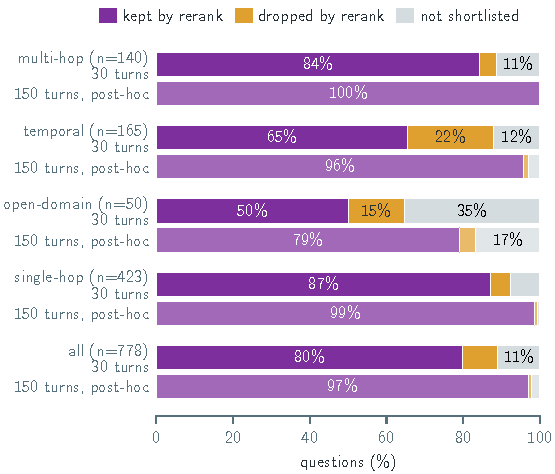
\includegraphics[width=\columnwidth]{figures/recall.pdf}
\caption{Where the evidence goes, by category, nine held-out conversations: missed by the 30-turn cosine shortlist, dropped by the rerank, or kept.}\label{fig:4}
\end{figure}
The categories differ. Open-domain evidence reaches the shortlist least often (63.0\%\src{bench/results/v3/shortlist\_recall.json\#all\_nine/by\_category/open-domain/shortlist\_recall\_any}) and is dropped most often (31.4\%\src{bench/results/v3/shortlist\_recall.json\#all\_nine/by\_category/open-domain/rerank\_drops\_all\_shortlisted\_evidence}), consistent with T0R trailing engram v2 on open-domain questions. Temporal evidence usually reaches the shortlist but is dropped by the rerank for 22.7\%\src{bench/results/v3/shortlist\_recall.json\#all\_nine/by\_category/temporal/rerank\_drops\_all\_shortlisted\_evidence} of questions: a turn that only establishes when something happened does not look relevant to the question on its own. Multi-hop questions usually get some evidence into the shortlist (88.4\%\src{bench/results/v3/shortlist\_recall.json\#all\_nine/by\_category/multi-hop/shortlist\_recall\_any}) but rarely all of it (42.8\%\src{bench/results/v3/shortlist\_recall.json\#all\_nine/by\_category/multi-hop/shortlist\_recall\_all}).

\textbf{A wider read path (post-hoc exploratory).} After the registered results were in, we tested one variant once, outside the Holm family and in its own ledger: T0R-wide takes a 150\src{bench/run.py\#ARMS/lean\_t0r\_wide/flags/retrieval\_shortlist}-turn cosine shortlist, asks Jev about every shortlisted turn, and keeps the top k by Jev's score with no cut-off, with $k{=}$47\src{bench/results/v3\_posthoc/report.json\#t0r\_wide\_k} matched to Jev-Mem at $k{=}$40 (2,000\src{bench/results/v3\_posthoc/report.json\#comparison/T0R-wide 47 (POST-HOC EXPLORATORY (T0R-wide; docs/V3\_PLAN.md §12))/tokens\_mean} tokens against 1,987\src{bench/results/v3\_posthoc/token\_match.json\#comparator\_mean\_tokens}). It scored 81.5\%\src{bench/results/v3\_posthoc/report.json\#comparison/T0R-wide 47 (POST-HOC EXPLORATORY (T0R-wide; docs/V3\_PLAN.md §12))/accuracy}, against 80.3\%\src{bench/results/v3/batch\_a\_report.json\#fresh/Jev-Mem k40/accuracy} for Jev-Mem at $k{=}$40 and 82.4\%\src{bench/results/v3/batch\_b\_report.json\#fresh/engram v2 k20/accuracy} for engram v2 at $k{=}$20 (1,238\src{bench/results/v3/batch\_b\_report.json\#fresh/engram v2 k20/tokens\_mean} tokens); all-evidence recall rose to 91.9\%\src{bench/results/v3\_posthoc/report.json\#shortlist\_recall/all/shortlist\_recall\_all} and the rerank's losses fell to 0.9\%\src{bench/results/v3\_posthoc/report.json\#shortlist\_recall/all/top\_k\_drops\_all\_shortlisted\_evidence}. This suggests the ceiling comes from T0R's read path rather than from storing raw turns, a hypothesis for new data, not a finding of this study.

\subsection{Cost and latency}\label{sec:5.7}
\begin{table*}[tbp]
\centering
\footnotesize\hyphenpenalty=10000\exhyphenpenalty=10000\setlength{\tabcolsep}{3.5pt}
\caption{Cost and latency (exploratory as registered). Write cost per 1,000 turns at list prices, split by LLM, Jev and embeddings; read cost per query; read latency measured live on a fixed sample of 40\src{docs/V3\_PLAN.md §7 (fixed sample of 40 questions); bench/v3\_latency.py} questions at $k{=}$3, one query at a time, including the query-embedding call. Jev-Mem's latency comes from its reads of the same questions, measured live when they ran (42\src{bench/results/v3/read\_latency\_live.json\#Jev-Mem (3, live at run time)/queries} reads: two question texts repeat).}\label{tab:5}
\begin{tabular}{@{}>{\raggedright\arraybackslash}p{60.3pt}>{\raggedleft\arraybackslash}p{33.9pt}>{\raggedleft\arraybackslash}p{29.4pt}>{\raggedleft\arraybackslash}p{29.4pt}>{\raggedleft\arraybackslash}p{52.5pt}>{\raggedleft\arraybackslash}p{31.6pt}>{\raggedleft\arraybackslash}p{38.4pt}>{\raggedright\arraybackslash}p{66.7pt}>{\raggedleft\arraybackslash}p{24.9pt}>{\raggedleft\arraybackslash}p{24.9pt}@{}}
\toprule
\textbf{System} & \textbf{Write \$/1k turns} & \textbf{LLM} & \textbf{Jev} & \textbf{Embeddings} & \textbf{Write p50 (s)} & \textbf{Read \$/query} & \textbf{Jev calls/query} & \textbf{Read p50 (ms)} & \textbf{Read p90 (ms)} \\
\midrule
T0R & \$0.0006\src{bench/results/v3/batch\_a\_report.json\#write/L0 / T0R (one store)/write\_cost\_per\_1k/embeddings} & -- & -- & \$0.0006\src{bench/results/v3/batch\_a\_report.json\#write/L0 / T0R (one store)/write\_cost\_per\_1k/embeddings} & 0.2\src{bench/results/v3/batch\_a\_report.json\#write/L0 / T0R (one store)/write\_latency\_p50\_ms\_by\_conv (median, s)} & \$0.00020\src{bench/results/v3/batch\_a\_report.json\#fresh/T0R k3/read\_cost\_per\_query} & one & 273\src{bench/results/v3/read\_latency\_live.json\#T0R/p50\_ms} & 359\src{bench/results/v3/read\_latency\_live.json\#T0R/p90\_ms} \\
L0 & \$0.0006\src{bench/results/v3/batch\_a\_report.json\#write/L0 / T0R (one store)/write\_cost\_per\_1k/embeddings} & -- & -- & \$0.0006\src{bench/results/v3/batch\_a\_report.json\#write/L0 / T0R (one store)/write\_cost\_per\_1k/embeddings} & 0.2\src{bench/results/v3/batch\_a\_report.json\#write/L0 / T0R (one store)/write\_latency\_p50\_ms\_by\_conv (median, s)} & -- & none & 219\src{bench/results/v3/read\_latency\_live.json\#L0/p50\_ms} & 263\src{bench/results/v3/read\_latency\_live.json\#L0/p90\_ms} \\
T0R-LLM & \$0.0006\src{bench/results/v3/batch\_a\_report.json\#write/L0 / T0R (one store)/write\_cost\_per\_1k/embeddings} & -- & -- & \$0.0006\src{bench/results/v3/batch\_a\_report.json\#write/L0 / T0R (one store)/write\_cost\_per\_1k/embeddings} & 0.2\src{bench/results/v3/batch\_a\_report.json\#write/L0 / T0R (one store)/write\_latency\_p50\_ms\_by\_conv (median, s)} & \$0.00023\src{bench/results/v3/batch\_b\_report.json\#fresh/T0R-LLM k3/read\_cost\_per\_query} & one (no-op) & 816\src{bench/results/v3/read\_latency\_live.json\#T0R-LLM/p50\_ms} & 1,107\src{bench/results/v3/read\_latency\_live.json\#T0R-LLM/p90\_ms} \\
engram v2 & \$1.865\src{bench/results/v3/batch\_b\_report.json\#write/engram v2/write\_cost\_per\_1k (sum)} & \$1.322\src{bench/results/v3/batch\_b\_report.json\#write/engram v2/write\_cost\_per\_1k (extraction + escalations + llm\_decisions)} & \$0.542\src{bench/results/v3/batch\_b\_report.json\#write/engram v2/write\_cost\_per\_1k/jev} & \$0.0015\src{bench/results/v3/batch\_b\_report.json\#write/engram v2/write\_cost\_per\_1k/embeddings} & 2.0\src{bench/results/v3/batch\_b\_report.json\#write/engram v2/write\_latency\_p50\_ms\_by\_conv (min, s)}--2.1\src{bench/results/v3/batch\_b\_report.json\#write/engram v2/write\_latency\_p50\_ms\_by\_conv (max, s)} & \$0.00018\src{bench/results/v3/batch\_b\_report.json\#fresh/engram v2 k3/read\_cost\_per\_query} & one & 276\src{bench/results/v3/read\_latency\_live.json\#engram v2/p50\_ms} & 319\src{bench/results/v3/read\_latency\_live.json\#engram v2/p90\_ms} \\
mem0 & \$1.321\src{bench/results/v3/batch\_b\_report.json\#write/mem0/write\_cost\_per\_1k (sum)} & \$1.319\src{bench/results/v3/batch\_b\_report.json\#write/mem0/write\_cost\_per\_1k (extraction + escalations + llm\_decisions)} & -- & \$0.0017\src{bench/results/v3/batch\_b\_report.json\#write/mem0/write\_cost\_per\_1k/embeddings} & 2.1\src{bench/results/v3/batch\_b\_report.json\#write/mem0/write\_latency\_p50\_ms\_by\_conv (min, s)}--2.3\src{bench/results/v3/batch\_b\_report.json\#write/mem0/write\_latency\_p50\_ms\_by\_conv (max, s)} & -- & none & 486\src{bench/results/v3/read\_latency\_live.json\#mem0/p50\_ms} & 718\src{bench/results/v3/read\_latency\_live.json\#mem0/p90\_ms} \\
Jev-Mem & \$0.211\src{bench/results/v3/batch\_a\_report.json\#write/Jev-Mem/write\_cost\_per\_1k/jev} & -- & \$0.211\src{bench/results/v3/batch\_a\_report.json\#write/Jev-Mem/write\_cost\_per\_1k/jev} & \$0.0011\src{bench/results/v3/batch\_a\_report.json\#write/Jev-Mem/write\_cost\_per\_1k/embeddings} & 0.5\src{bench/results/v3/batch\_a\_report.json\#write/Jev-Mem/write\_latency\_p50\_ms\_by\_conv (median, s)} & \$0.00120\src{bench/results/v3/batch\_a\_report.json\#fresh/Jev-Mem k3/read\_cost\_per\_query} & 5.3\src{bench/results/v3/batch\_a\_report.json\#jevmem\_reads/k3/jev\_calls\_mean} & 1,329\src{bench/results/v3/read\_latency\_live.json\#Jev-Mem (3, live at run time)/p50\_ms} & 1,622\src{bench/results/v3/read\_latency\_live.json\#Jev-Mem (3, live at run time)/p90\_ms} \\
\bottomrule
\end{tabular}
\end{table*}
Jev reads about 3.0\src{bench/results/v3/read\_latency\_live.json (T0R-LLM p50 / T0R p50)}$\times$ faster than the LLM reranker and 4.9\src{bench/results/v3/read\_latency\_live.json (Jev-Mem p50 / T0R p50)}$\times$ faster than Jev-Mem at $k{=}$3; engram v2 reads as fast as T0R because its read path is the same one request. The write cost is where the systems differ: extraction makes engram v2 and mem0 thousands of times more expensive to write than T0R, and Jev-Mem's two Jev requests per turn cost \$0.211\src{bench/results/v3/batch\_a\_report.json\#write/Jev-Mem/write\_cost\_per\_1k/jev} per 1,000 turns. Jev-Mem at $k{=}$40 averaged 3.0\src{bench/results/v3/batch\_a\_report.json\#jevmem\_reads/k40/jev\_calls\_mean} Jev calls per query (up to 11\src{bench/results/v3/batch\_a\_report.json\#jevmem\_reads/k40/jev\_calls\_max}) and \$0.00174\src{bench/results/v3/batch\_a\_report.json\#fresh/Jev-Mem k40/read\_cost\_per\_query} per query. Mem0's read cost is a query embedding only.

\begin{figure}[tbp]
\centering
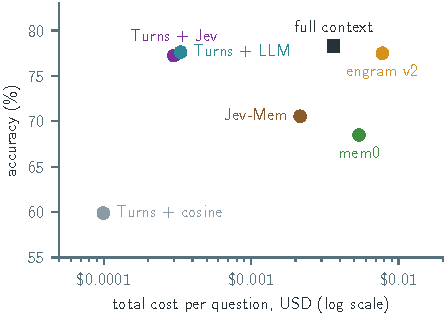
\includegraphics[width=\columnwidth]{figures/cost.pdf}
\caption{Accuracy against total cost per question (log scale), five held-out conversations: write cost amortised at the benchmark's ratio of about 4 turns written per question asked (filled), and at one turn per question, a read-heavy use (hollow), plus read cost and answer cost (judge excluded), at list prices.}\label{fig:5}
\end{figure}
Figure~\ref{fig:5} amortises write cost at the benchmark's own ratio (4.0\src{bench/results/v3/batch\_b\_report.json\#write/engram v2/turns / 778} turns written per scored question). At that ratio T0R's total cost per question is \$0.00030\src{write per 1k x bench turns per question / 1000 + mean query\_cost of lean\_t0r\_\_k3} and engram v2's \$0.00778\src{write per 1k x bench turns per question / 1000 + mean query\_cost of e4\_frozen\_sameattr\_\_k3}; full context costs \$0.00362\src{write per 1k x bench turns per question / 1000 + mean query\_cost of full\_context}. In a read-heavy use with one turn written per question, the write cost weighs less: engram v2's total falls to \$0.00216\src{write per 1k x read\_heavy turns per question / 1000 + mean query\_cost of e4\_frozen\_sameattr\_\_k3}.

\subsection{Abstention}\label{sec:5.8}
\begin{table}[tbp]
\centering
\footnotesize\hyphenpenalty=10000\exhyphenpenalty=10000\setlength{\tabcolsep}{6.0pt}
\caption{Share of LoCoMo adversarial questions (209\src{bench/results/v3/batch\_b\_report.json\#fresh\_adversarial/mem0 k3/questions}, five held-out conversations) answered by abstaining (exploratory as registered).}\label{tab:6}
\begin{tabular}{@{}>{\raggedright\arraybackslash}p{110.5pt}>{\raggedleft\arraybackslash}p{42.2pt}>{\raggedleft\arraybackslash}p{42.2pt}@{}}
\toprule
\textbf{System} & \textbf{$k{=}$3} & \textbf{$k{=}$20} \\
\midrule
L0 & 63.6\%\src{bench/results/v3/batch\_a\_report.json\#fresh\_adversarial/L0 k3/abstained} & 47.8\%\src{bench/results/v3/batch\_a\_report.json\#fresh\_adversarial/L0 k20/abstained} \\
engram v2 & 59.8\%\src{bench/results/v3/batch\_b\_report.json\#fresh\_adversarial/engram v2 k3/abstained} & 52.2\%\src{bench/results/v3/batch\_b\_report.json\#fresh\_adversarial/engram v2 k20/abstained} \\
mem0 & 59.8\%\src{bench/results/v3/batch\_b\_report.json\#fresh\_adversarial/mem0 k3/abstained} & 53.6\%\src{bench/results/v3/batch\_b\_report.json\#fresh\_adversarial/mem0 k20/abstained} \\
T0R & 54.1\%\src{bench/results/v3/batch\_a\_report.json\#fresh\_adversarial/T0R k3/abstained} & 49.3\%\src{bench/results/v3/batch\_a\_report.json\#fresh\_adversarial/T0R k20/abstained} \\
T0R-LLM & 48.8\%\src{bench/results/v3/batch\_b\_report.json\#fresh\_adversarial/T0R-LLM k3/abstained} & 53.1\%\src{bench/results/v3/batch\_b\_report.json\#fresh\_adversarial/T0R-LLM k20/abstained} \\
\bottomrule
\end{tabular}
\end{table}
Reranking lowered correct abstention at $k{=}$3, with Jev (54.1\%\src{bench/results/v3/batch\_a\_report.json\#fresh\_adversarial/T0R k3/abstained}) and with an LLM reranker (48.8\%\src{bench/results/v3/batch\_b\_report.json\#fresh\_adversarial/T0R-LLM k3/abstained}) against similarity search (63.6\%\src{bench/results/v3/batch\_a\_report.json\#fresh\_adversarial/L0 k3/abstained}): relevant-looking context makes the answer model less willing to say that something was not mentioned. The exploratory conversations show the same (54.2\%\src{bench/results/v3/batch\_a\_report.json\#exploratory/adversarial/T0R k3/abstained} against 65.3\%\src{bench/results/v3/batch\_a\_report.json\#exploratory/adversarial/L0 k3/abstained}), and so does LongMemEval at $k{=}$20 (63.3\%\src{bench/results/v3/batch\_c\_report.json\#expansion/T0R 20 (abstention, correct = abstained)/accuracy} for T0R against 70.0\%\src{bench/results/v3/batch\_c\_report.json\#expansion/L0 20 (abstention, correct = abstained)/accuracy} for L0). Fidelity Before Structure reports that verbatim chunks abstain worse than extracted artifacts; we find that reranking specifically adds to that.

\section{Discussion}\label{sec:6}
\textbf{A budget reading of two prior findings (interpretation).} SmartSearch finds ranking to be the bottleneck; Fidelity finds reranking marginal. Our within-study results suggest the difference is the budget: reranking matters in proportion to how hard truncation cuts the candidate set. In SmartSearch a question has about 431\src{cite:derehag2026smartsearch (checked against the paper's text; paper\_v3/bib\_verification.md)} grep candidates on average, of which about 62\src{cite:derehag2026smartsearch (checked against the paper's text; paper\_v3/bib\_verification.md)} passages fit its 2,000\src{cite:derehag2026smartsearch (checked against the paper's text; paper\_v3/bib\_verification.md)}-word budget, and without ranking only 22.5\src{cite:derehag2026smartsearch (checked against the paper's text; paper\_v3/bib\_verification.md)}\% of gold evidence survives truncation; our $k{=}$3 keeps three of 30\src{docs/V3\_PLAN.md §1, §2, §4}. Both show large ranking gains. Fidelity reranks a top-30\src{cite:an2026fidelity (checked against the paper's text; paper\_v3/bib\_verification.md)} pool to 15\src{cite:an2026fidelity (checked against the paper's text; paper\_v3/bib\_verification.md)} with bge-reranker-v2-m3 under a 5,000\src{cite:an2026fidelity (checked against the paper's text; paper\_v3/bib\_verification.md)}-token cap (gains of 2.9\src{cite:an2026fidelity (checked against the paper's text; paper\_v3/bib\_verification.md)} points on LoCoMo and 0.6\src{cite:an2026fidelity (checked against the paper's text; paper\_v3/bib\_verification.md)} on LongMemEval-S), and our $k{=}$20 keeps twenty of 30\src{docs/V3\_PLAN.md §1, §2, §4}; both show small ones. This is an interpretation across pipelines that differ in retrievers, rerankers, answer models and judges, supported inside our study by the $k{=}$3 to $k{=}$20 comparison on two benchmarks, not a tested claim across papers.

\textbf{When extraction is worth it.} At the tight budget of H1, extraction adds little and costs thousands of times more to write. At generous budgets it is more accurate and more compact: engram v2 at $k{=}$20 was the most accurate system we measured, with fewer tokens than Jev-Mem at $k{=}$40. Open-domain and temporal questions are where T0R trailed engram v2, and where its shortlist and rerank lose the most evidence.

\textbf{What a typed decision model contributes.} In this study, speed and cost at equal selection quality, not higher accuracy: Jev selected as accurately as the gpt-4o-mini reranker (S4) at about a third of the latency, in one request per question, and one Jev request beat Jev-Mem's multi-request graph walk at matched context (S2). A typed question returns a probability over fixed options in one short call, which is what a reranker needs.

\textbf{Judge leniency and answer style.} mem0's LoCoMo judge is lenient, and in our audit it credited short answers more readily than list-style ones, so its agreement with human grading differed by system. Memory benchmarks that compare systems with different answer styles should report judge--human agreement by system.

\textbf{Not state of the art.} SmartSearch reports 91.9\src{cite:derehag2026smartsearch (checked against the paper's text; paper\_v3/bib\_verification.md)}\% on LoCoMo under its own protocol (gpt-4o-mini answering and judging, binary judgments, all ten conversations and 1,540\src{cite:derehag2026smartsearch (checked against the paper's text; paper\_v3/bib\_verification.md)} questions in categories 1--4, 3,141\src{cite:derehag2026smartsearch (checked against the paper's text; paper\_v3/bib\_verification.md)} tokens per question); our numbers come from a different protocol and five held-out conversations and are not comparable to it. Our best result, the post-hoc T0R-wide, is below that figure.

\section*{Limitations}
\begin{itemize}
\item \textbf{Benchmarks.} One benchmark family per setting: LoCoMo, whose dialogues are LLM-generated, and LongMemEval. Five primary conversations give 778\src{bench/results/v3/batch\_b\_report.json\#H1/questions} questions; categories are small.
\item \textbf{LongMemEval scope.} engram v2 was not run on LongMemEval, so no claim about extraction on long histories follows from this study.
\item \textbf{Human grading.} The grader is the system's author; the mapping of partial grades was not pre-specified (two are reported); one question was ungraded; and only judge-discordant questions were re-graded, so judge errors on questions where the judge agreed across systems remain.
\item \textbf{A closed decision model.} Jev is a closed, versioned model; results hold for jev-1.13.0.
\item \textbf{mem0 serving.} mem0's extraction calls were served through OpenRouter, about half by Azure, not the OpenAI API as registered; only S3 involves mem0.
\item \textbf{Post-hoc variant.} T0R-wide was designed after the registered results and tested once on the same questions.
\item \textbf{Absolute accuracy.} Below SmartSearch's reported figures at generous budgets, under a different protocol.
\item \textbf{Development data.} Every design choice was made on one conversation, conv-26.
\end{itemize}
\section{Conclusion}\label{sec:7}
At tight context budgets, raw conversation turns reranked by one call to a typed decision model were non-inferior within a 5\src{docs/V3\_PLAN.md §1, §2, §4}-point margin to LLM-extracted memory, at thousands of times lower write cost, on held-out conversations, two answer models and blind human grading. The value of that rerank depends on the budget: large when three of 30\src{docs/V3\_PLAN.md §1, §2, §4} candidates are kept, small when twenty are. Jev selected as accurately as an LLM reranker at about a third of the latency. At generous budgets extraction systems were more accurate, so the result is a statement about tight budgets.

\section*{AI Assistance}
The code, run orchestration and drafting of this paper were done with Claude Code (Anthropic) under the author's direction. The author made every methodological decision, approved each stage of the registered plan and did the human audit.

\section*{Artifacts}
Code, plans, per-question answers and judge labels, and the human-audit grades with their key are at github.com/ris3abh/Engram: tags \texttt{v3-frozen}, \texttt{v3-amended} and the paper tag; results in \texttt{bench/\allowbreak{}results/\allowbreak{}v3/\allowbreak{}} (per-question files, reports, ledgers, \texttt{human\_\allowbreak{}audit/\allowbreak{}}) and \texttt{bench/\allowbreak{}results/\allowbreak{}v3\_\allowbreak{}posthoc/\allowbreak{}}. The plan and its amendment are deposited at 10.5281/zenodo.22970745 and 10.5281/zenodo.22977848; the earlier engram preprint is 10.5281/zenodo.22941757 \citep{sharma2026typed}.

\bibliography{references}
\appendix
\onecolumn
\FloatBarrier
\section{Per-conversation results}\label{app:A}
\begin{table}[!htbp]
\centering
\footnotesize\hyphenpenalty=10000\exhyphenpenalty=10000\setlength{\tabcolsep}{6.0pt}
\caption{Accuracy (\%) per conversation, LoCoMo scored categories.}
\begin{tabular}{@{}>{\raggedright\arraybackslash}p{165.3pt}>{\raggedleft\arraybackslash}p{45.9pt}>{\raggedleft\arraybackslash}p{45.9pt}>{\raggedleft\arraybackslash}p{45.9pt}>{\raggedleft\arraybackslash}p{45.9pt}>{\raggedleft\arraybackslash}p{45.9pt}@{}}
\toprule
\textbf{System, setting} & \textbf{conv-44 (123\src{bench/results/v3/lean\_t0r\_\_heldout\_conv-44\_\_k3.json\#answers (count)})} & \textbf{conv-47 (150\src{bench/results/v3/lean\_t0r\_\_heldout\_conv-47\_\_k3.json\#answers (count)})} & \textbf{conv-48 (191\src{bench/results/v3/lean\_t0r\_\_heldout\_conv-48\_\_k3.json\#answers (count)})} & \textbf{conv-49 (156\src{bench/results/v3/lean\_t0r\_\_heldout\_conv-49\_\_k3.json\#answers (count)})} & \textbf{conv-50 (158\src{bench/results/v3/lean\_t0r\_\_heldout\_conv-50\_\_k3.json\#answers (count)})} \\
\midrule
T0R, $k{=}$3 & 78.0\src{bench/results/v3/lean\_t0r\_\_heldout\_conv-44\_\_k3.json\#answers (share CORRECT)} & 76.7\src{bench/results/v3/lean\_t0r\_\_heldout\_conv-47\_\_k3.json\#answers (share CORRECT)} & 79.1\src{bench/results/v3/lean\_t0r\_\_heldout\_conv-48\_\_k3.json\#answers (share CORRECT)} & 73.7\src{bench/results/v3/lean\_t0r\_\_heldout\_conv-49\_\_k3.json\#answers (share CORRECT)} & 78.5\src{bench/results/v3/lean\_t0r\_\_heldout\_conv-50\_\_k3.json\#answers (share CORRECT)} \\
T0R, $k{=}$6 & 79.7\src{bench/results/v3/lean\_t0r\_\_heldout\_conv-44\_\_k6.json\#answers (share CORRECT)} & 76.7\src{bench/results/v3/lean\_t0r\_\_heldout\_conv-47\_\_k6.json\#answers (share CORRECT)} & 78.5\src{bench/results/v3/lean\_t0r\_\_heldout\_conv-48\_\_k6.json\#answers (share CORRECT)} & 73.7\src{bench/results/v3/lean\_t0r\_\_heldout\_conv-49\_\_k6.json\#answers (share CORRECT)} & 76.6\src{bench/results/v3/lean\_t0r\_\_heldout\_conv-50\_\_k6.json\#answers (share CORRECT)} \\
T0R, $k{=}$20 & 79.7\src{bench/results/v3/lean\_t0r\_\_heldout\_conv-44\_\_k20.json\#answers (share CORRECT)} & 74.7\src{bench/results/v3/lean\_t0r\_\_heldout\_conv-47\_\_k20.json\#answers (share CORRECT)} & 81.7\src{bench/results/v3/lean\_t0r\_\_heldout\_conv-48\_\_k20.json\#answers (share CORRECT)} & 75.0\src{bench/results/v3/lean\_t0r\_\_heldout\_conv-49\_\_k20.json\#answers (share CORRECT)} & 76.6\src{bench/results/v3/lean\_t0r\_\_heldout\_conv-50\_\_k20.json\#answers (share CORRECT)} \\
L0, $k{=}$3 & 65.9\src{bench/results/v3/lean\_l0\_\_heldout\_conv-44\_\_k3.json\#answers (share CORRECT)} & 57.3\src{bench/results/v3/lean\_l0\_\_heldout\_conv-47\_\_k3.json\#answers (share CORRECT)} & 62.8\src{bench/results/v3/lean\_l0\_\_heldout\_conv-48\_\_k3.json\#answers (share CORRECT)} & 58.3\src{bench/results/v3/lean\_l0\_\_heldout\_conv-49\_\_k3.json\#answers (share CORRECT)} & 55.7\src{bench/results/v3/lean\_l0\_\_heldout\_conv-50\_\_k3.json\#answers (share CORRECT)} \\
L0, $k{=}$20 & 78.0\src{bench/results/v3/lean\_l0\_\_heldout\_conv-44\_\_k20.json\#answers (share CORRECT)} & 74.0\src{bench/results/v3/lean\_l0\_\_heldout\_conv-47\_\_k20.json\#answers (share CORRECT)} & 79.1\src{bench/results/v3/lean\_l0\_\_heldout\_conv-48\_\_k20.json\#answers (share CORRECT)} & 74.4\src{bench/results/v3/lean\_l0\_\_heldout\_conv-49\_\_k20.json\#answers (share CORRECT)} & 74.7\src{bench/results/v3/lean\_l0\_\_heldout\_conv-50\_\_k20.json\#answers (share CORRECT)} \\
T0R-LLM, $k{=}$3 & 76.4\src{bench/results/v3/lean\_t0r\_llm\_\_heldout\_conv-44\_\_k3.json\#answers (share CORRECT)} & 72.7\src{bench/results/v3/lean\_t0r\_llm\_\_heldout\_conv-47\_\_k3.json\#answers (share CORRECT)} & 80.6\src{bench/results/v3/lean\_t0r\_llm\_\_heldout\_conv-48\_\_k3.json\#answers (share CORRECT)} & 77.6\src{bench/results/v3/lean\_t0r\_llm\_\_heldout\_conv-49\_\_k3.json\#answers (share CORRECT)} & 79.7\src{bench/results/v3/lean\_t0r\_llm\_\_heldout\_conv-50\_\_k3.json\#answers (share CORRECT)} \\
engram v2, $k{=}$3 & 77.2\src{bench/results/v3/e4\_frozen\_sameattr\_\_heldout\_conv-44\_\_k3.json\#answers (share CORRECT)} & 80.7\src{bench/results/v3/e4\_frozen\_sameattr\_\_heldout\_conv-47\_\_k3.json\#answers (share CORRECT)} & 78.5\src{bench/results/v3/e4\_frozen\_sameattr\_\_heldout\_conv-48\_\_k3.json\#answers (share CORRECT)} & 76.3\src{bench/results/v3/e4\_frozen\_sameattr\_\_heldout\_conv-49\_\_k3.json\#answers (share CORRECT)} & 74.7\src{bench/results/v3/e4\_frozen\_sameattr\_\_heldout\_conv-50\_\_k3.json\#answers (share CORRECT)} \\
engram v2, $k{=}$20 & 84.6\src{bench/results/v3/e4\_frozen\_sameattr\_\_heldout\_conv-44\_\_k20.json\#answers (share CORRECT)} & 84.7\src{bench/results/v3/e4\_frozen\_sameattr\_\_heldout\_conv-47\_\_k20.json\#answers (share CORRECT)} & 82.2\src{bench/results/v3/e4\_frozen\_sameattr\_\_heldout\_conv-48\_\_k20.json\#answers (share CORRECT)} & 80.8\src{bench/results/v3/e4\_frozen\_sameattr\_\_heldout\_conv-49\_\_k20.json\#answers (share CORRECT)} & 80.4\src{bench/results/v3/e4\_frozen\_sameattr\_\_heldout\_conv-50\_\_k20.json\#answers (share CORRECT)} \\
mem0, $k{=}$3 & 68.3\src{bench/results/v3/mem0\_\_heldout\_conv-44\_\_k3.json\#answers (share CORRECT)} & 65.3\src{bench/results/v3/mem0\_\_heldout\_conv-47\_\_k3.json\#answers (share CORRECT)} & 69.6\src{bench/results/v3/mem0\_\_heldout\_conv-48\_\_k3.json\#answers (share CORRECT)} & 72.4\src{bench/results/v3/mem0\_\_heldout\_conv-49\_\_k3.json\#answers (share CORRECT)} & 66.5\src{bench/results/v3/mem0\_\_heldout\_conv-50\_\_k3.json\#answers (share CORRECT)} \\
mem0, $k{=}$20 & 79.7\src{bench/results/v3/mem0\_\_heldout\_conv-44\_\_k20.json\#answers (share CORRECT)} & 78.0\src{bench/results/v3/mem0\_\_heldout\_conv-47\_\_k20.json\#answers (share CORRECT)} & 81.2\src{bench/results/v3/mem0\_\_heldout\_conv-48\_\_k20.json\#answers (share CORRECT)} & 78.8\src{bench/results/v3/mem0\_\_heldout\_conv-49\_\_k20.json\#answers (share CORRECT)} & 75.3\src{bench/results/v3/mem0\_\_heldout\_conv-50\_\_k20.json\#answers (share CORRECT)} \\
Jev-Mem, $k{=}$3 & 69.1\src{bench/results/v3/jevmem\_\_heldout\_conv-44\_\_k3.json\#answers (share CORRECT)} & 66.7\src{bench/results/v3/jevmem\_\_heldout\_conv-47\_\_k3.json\#answers (share CORRECT)} & 74.3\src{bench/results/v3/jevmem\_\_heldout\_conv-48\_\_k3.json\#answers (share CORRECT)} & 69.2\src{bench/results/v3/jevmem\_\_heldout\_conv-49\_\_k3.json\#answers (share CORRECT)} & 72.2\src{bench/results/v3/jevmem\_\_heldout\_conv-50\_\_k3.json\#answers (share CORRECT)} \\
Jev-Mem, $k{=}$40 & 81.3\src{bench/results/v3/jevmem\_\_heldout\_conv-44\_\_k40.json\#answers (share CORRECT)} & 78.7\src{bench/results/v3/jevmem\_\_heldout\_conv-47\_\_k40.json\#answers (share CORRECT)} & 80.6\src{bench/results/v3/jevmem\_\_heldout\_conv-48\_\_k40.json\#answers (share CORRECT)} & 82.7\src{bench/results/v3/jevmem\_\_heldout\_conv-49\_\_k40.json\#answers (share CORRECT)} & 78.5\src{bench/results/v3/jevmem\_\_heldout\_conv-50\_\_k40.json\#answers (share CORRECT)} \\
Full context & 82.1\src{bench/results/v3/full\_context\_\_heldout\_conv-44.json\#answers (share CORRECT)} & 72.7\src{bench/results/v3/full\_context\_\_heldout\_conv-47.json\#answers (share CORRECT)} & 82.7\src{bench/results/v3/full\_context\_\_heldout\_conv-48.json\#answers (share CORRECT)} & 76.3\src{bench/results/v3/full\_context\_\_heldout\_conv-49.json\#answers (share CORRECT)} & 77.2\src{bench/results/v3/full\_context\_\_heldout\_conv-50.json\#answers (share CORRECT)} \\
\bottomrule
\end{tabular}
\end{table}
The exploratory replication on conv-30, conv-41, conv-42 and conv-43 (610\src{bench/results/v3/batch\_a\_report.json\#exploratory/L0 k3/questions} scored questions): L0 60.7\%\src{bench/results/v3/batch\_a\_report.json\#exploratory/L0 k3/accuracy} at $k{=}$3 and 76.2\%\src{bench/results/v3/batch\_a\_report.json\#exploratory/L0 k20/accuracy} at $k{=}$20; T0R 77.2\%\src{bench/results/v3/batch\_a\_report.json\#exploratory/T0R k3/accuracy} at $k{=}$3 and 76.6\%\src{bench/results/v3/batch\_a\_report.json\#exploratory/T0R k20/accuracy} at $k{=}$20. T0R's matched k against L0 was 3\src{bench/results/v3/batch\_a\_report.json\#token\_match/L0 (exploratory)/t0r\_k}, with 116\src{bench/results/v3/batch\_a\_report.json\#exploratory/T0R vs L0 (matched)/only\_a} questions correct only for T0R and 15\src{bench/results/v3/batch\_a\_report.json\#exploratory/T0R vs L0 (matched)/only\_b} only for L0 (p = 1.6e$-$20\src{bench/results/v3/batch\_a\_report.json\#exploratory/T0R vs L0 (matched)/p\_two\_sided}, exploratory).

\FloatBarrier
\section{Registered plan and deviations}\label{app:B}
The plan (its guarded sections in \texttt{docs/\allowbreak{}V3\_\allowbreak{}PLAN.md}, checked by a test that fails on any undated change, fixed the systems, data, token-matching rule, tests, predictions, human check, run order and budget before any run. Every change is a dated entry in its Deviations section:

\begin{itemize}
\item \textbf{2026-09-26, amendment}, deposited before any primary-test result was seen: shortlist recall; LongMemEval on all 500\src{bench/results/v3/batch\_c\_report.json (470 scored + 30 abstention)} questions with user and assistant turns and the new test S7; the second answer model; the outcome paragraphs and the rule for ``LongMemEval holds''; budget caps.
\item \textbf{2026-09-26, outcome paragraphs revised} before upload, before any primary-test result was seen.
\item \textbf{2026-09-26, Batch B execution}: mem0's extraction was routed to OpenRouter by a library default (\hyperref[app:G]{Appendix~G}); runs hit OpenAI's rate limit and were repeated with more retries and a Jev throttle, completed calls replaying from a call cache; T0R-LLM also asks Jev one query-relation question per query, a no-op on turns.
\item \textbf{2026-09-26, mem0 via OpenRouter resolved}: model and serving provider established, billed amount corrected in the ledger, guards added before any later run.
\item \textbf{2026-09-27, human check layout} (record only): each answer on its own row, all 284\src{bench/results/v3/human\_audit/audit\_report.json\#rows} rows shuffled together, rather than randomising the order within each question.
\item \textbf{2026-09-27, human check grading standard} (record only): the sheet asked for CORRECT or WRONG; partial grades appeared, so two mappings are reported.
\item \textbf{2026-09-27, paper title} (presentation change): the title the outcome rule selected, ``Selection, Not Extraction: One Rerank Call Matches LLM-Extracted Memory at a Fraction of the Write Cost'', was replaced because it presents a published idea as new and its ``matches'' overstates a non-inferiority result.
\end{itemize}
Implementation notes not in the Deviations section: one LongMemEval haystack contains the literal text \texttt{\textless{}|endoftext|\textgreater{}}, which the token counter refused; counting now treats it as ordinary text, and the affected question was re-run. Two retrieval-only sweeps were stopped by mistake and re-run from the cache.

\FloatBarrier
\section{Human audit}\label{app:C}
\textbf{Protocol.} The sheet held every question on which the judge found exactly one of H1's two answers correct (142\src{bench/results/v3/batch\_b\_report.json\#H1 (only\_a + only\_b)} questions), each answer as its own row (284\src{bench/results/v3/human\_audit/audit\_report.json\#rows} rows), shuffled with seed 0, with the question and gold answer shown and no system name or judge label. The sheet asked for CORRECT or WRONG; the plan's notes had listed CORRECT, WRONG or UNCLEAR. The author's grades included partial and hedged labels, and one question was left ungraded. Two mappings are reported: strict (only grades starting with CORRECT count as correct) and lenient (partial and hedged-correct grades also count); any grade containing WRONG counts as wrong under both. H1 is decided by the judge.

\begin{table}[!htbp]
\centering
\footnotesize\hyphenpenalty=10000\exhyphenpenalty=10000\setlength{\tabcolsep}{4.5pt}

\begin{tabular}{@{}>{\raggedright\arraybackslash}p{115.8pt}>{\raggedleft\arraybackslash}p{53.6pt}>{\raggedleft\arraybackslash}p{44.4pt}>{\raggedleft\arraybackslash}p{44.4pt}>{\raggedleft\arraybackslash}p{29.1pt}>{\raggedleft\arraybackslash}p{39.9pt}>{\raggedleft\arraybackslash}p{29.1pt}>{\raggedleft\arraybackslash}p{35.4pt}@{}}
\toprule
\textbf{Mapping} & \textbf{Agreement with judge} & \textbf{On T0R's answers} & \textbf{On engram v2's answers} & \textbf{Only T0R right} & \textbf{Only engram v2 right} & \textbf{Both right} & \textbf{Both wrong} \\
\midrule
Strict & 81\%\src{bench/results/v3/human\_audit/audit\_report.json\#strict/agreement\_with\_judge} & 81\%\src{bench/results/v3/human\_audit/audit\_report.json\#strict/agreement\_with\_judge\_by\_system/T0R} & 82\%\src{bench/results/v3/human\_audit/audit\_report.json\#strict/agreement\_with\_judge\_by\_system/engram} & 47\src{bench/results/v3/human\_audit/audit\_report.json\#strict/human\_only\_t0r} & 59\src{bench/results/v3/human\_audit/audit\_report.json\#strict/human\_only\_engram} & 17\src{bench/results/v3/human\_audit/audit\_report.json\#strict/human\_both\_correct} & 18\src{bench/results/v3/human\_audit/audit\_report.json\#strict/human\_both\_wrong} \\
Lenient & 79\%\src{bench/results/v3/human\_audit/audit\_report.json\#lenient/agreement\_with\_judge} & 82\%\src{bench/results/v3/human\_audit/audit\_report.json\#lenient/agreement\_with\_judge\_by\_system/T0R} & 77\%\src{bench/results/v3/human\_audit/audit\_report.json\#lenient/agreement\_with\_judge\_by\_system/engram} & 41\src{bench/results/v3/human\_audit/audit\_report.json\#lenient/human\_only\_t0r} & 60\src{bench/results/v3/human\_audit/audit\_report.json\#lenient/human\_only\_engram} & 31\src{bench/results/v3/human\_audit/audit\_report.json\#lenient/human\_both\_correct} & 9\src{bench/results/v3/human\_audit/audit\_report.json\#lenient/human\_both\_wrong} \\
\bottomrule
\end{tabular}
\end{table}
The grades, the key and the analysis are in \texttt{bench/\allowbreak{}results/\allowbreak{}v3/\allowbreak{}human\_\allowbreak{}audit/\allowbreak{}} and \texttt{bench/\allowbreak{}v3\_\allowbreak{}human\_\allowbreak{}audit.py}.

\FloatBarrier
\section{Shortlist recall}\label{app:D}
For every scored question of the nine held-out conversations, the 30\src{docs/V3\_PLAN.md §1, §2, §4}-turn cosine shortlist (shared by L0 and T0R) and the turns T0R's rerank keeps were rebuilt from the frozen stores through the call cache. Each turn's id is its LoCoMo dialogue id, so the question's evidence ids can be located. Reported: the share of questions with all, and with at least one, evidence turn in the shortlist, and, among questions with an evidence turn in the shortlist, the share where the rerank keeps none. Recall is scored on raw turns only \citep{samerank2026}. The five fresh conversations (76.9\%\src{bench/results/v3/shortlist\_recall.json\#fresh\_five/all/shortlist\_recall\_all} all-evidence recall, 10.4\%\src{bench/results/v3/shortlist\_recall.json\#fresh\_five/all/rerank\_drops\_all\_shortlisted\_evidence} dropped by the rerank) and the four exploratory ones (76.9\%\src{bench/results/v3/shortlist\_recall.json\#exploratory\_four/all/shortlist\_recall\_all}, 10.3\%\src{bench/results/v3/shortlist\_recall.json\#exploratory\_four/all/rerank\_drops\_all\_shortlisted\_evidence}) agree.

\begin{table}[!htbp]
\centering
\footnotesize\hyphenpenalty=10000\exhyphenpenalty=10000\setlength{\tabcolsep}{6.0pt}

\begin{tabular}{@{}>{\raggedright\arraybackslash}p{185.4pt}>{\raggedleft\arraybackslash}p{63.0pt}>{\raggedleft\arraybackslash}p{58.3pt}>{\raggedleft\arraybackslash}p{47.3pt}>{\raggedleft\arraybackslash}p{53.1pt}@{}}
\toprule
\textbf{Category} & \textbf{Questions} & \textbf{All evidence in shortlist} & \textbf{At least one} & \textbf{Rerank keeps none} \\
\midrule
Multi-hop & 250\src{bench/results/v3/shortlist\_recall.json\#all\_nine/by\_category/multi-hop/questions} & 42.8\%\src{bench/results/v3/shortlist\_recall.json\#all\_nine/by\_category/multi-hop/shortlist\_recall\_all} & 88.4\%\src{bench/results/v3/shortlist\_recall.json\#all\_nine/by\_category/multi-hop/shortlist\_recall\_any} & 5.9\%\src{bench/results/v3/shortlist\_recall.json\#all\_nine/by\_category/multi-hop/rerank\_drops\_all\_shortlisted\_evidence} \\
Temporal & 284\src{bench/results/v3/shortlist\_recall.json\#all\_nine/by\_category/temporal/questions} & 83.5\%\src{bench/results/v3/shortlist\_recall.json\#all\_nine/by\_category/temporal/shortlist\_recall\_all} & 88.4\%\src{bench/results/v3/shortlist\_recall.json\#all\_nine/by\_category/temporal/shortlist\_recall\_any} & 22.7\%\src{bench/results/v3/shortlist\_recall.json\#all\_nine/by\_category/temporal/rerank\_drops\_all\_shortlisted\_evidence} \\
Open-domain & 83\src{bench/results/v3/shortlist\_recall.json\#all\_nine/by\_category/open-domain/questions} & 42.0\%\src{bench/results/v3/shortlist\_recall.json\#all\_nine/by\_category/open-domain/shortlist\_recall\_all} & 63.0\%\src{bench/results/v3/shortlist\_recall.json\#all\_nine/by\_category/open-domain/shortlist\_recall\_any} & 31.4\%\src{bench/results/v3/shortlist\_recall.json\#all\_nine/by\_category/open-domain/rerank\_drops\_all\_shortlisted\_evidence} \\
Single-hop & 771\src{bench/results/v3/shortlist\_recall.json\#all\_nine/by\_category/single-hop/questions} & 89.2\%\src{bench/results/v3/shortlist\_recall.json\#all\_nine/by\_category/single-hop/shortlist\_recall\_all} & 91.2\%\src{bench/results/v3/shortlist\_recall.json\#all\_nine/by\_category/single-hop/shortlist\_recall\_any} & 5.8\%\src{bench/results/v3/shortlist\_recall.json\#all\_nine/by\_category/single-hop/rerank\_drops\_all\_shortlisted\_evidence} \\
All & 1,388\src{bench/results/v3/shortlist\_recall.json\#all\_nine/all/questions} & 76.9\%\src{bench/results/v3/shortlist\_recall.json\#all\_nine/all/shortlist\_recall\_all} & 88.5\%\src{bench/results/v3/shortlist\_recall.json\#all\_nine/all/shortlist\_recall\_any} & 10.4\%\src{bench/results/v3/shortlist\_recall.json\#all\_nine/all/rerank\_drops\_all\_shortlisted\_evidence} \\
\bottomrule
\end{tabular}
\end{table}
\FloatBarrier
\section{T0R-wide (post-hoc exploratory)}\label{app:E}
Designed after the registered results were seen, tested once on the 778\src{bench/results/v3/batch\_b\_report.json\#H1/questions} questions of the five held-out conversations, outside the Holm family, in its own ledger (\$0.31\src{bench/results/v3\_posthoc/report.json\#ledger/openai} OpenAI and \$0.58\src{bench/results/v3\_posthoc/report.json\#ledger/jev} Jev). Design: T0R's store; a 150\src{bench/run.py\#ARMS/lean\_t0r\_wide/flags/retrieval\_shortlist}-turn cosine shortlist; Jev's relevance question on every shortlisted turn, thirty per request; the top k by Jev's probability, with no cut-off, floor or expansion; $k{=}$47\src{bench/results/v3\_posthoc/report.json\#t0r\_wide\_k} matched to Jev-Mem at $k{=}$40 by the registered rule, saved before answering. Results: accuracy 81.5\%\src{bench/results/v3\_posthoc/report.json\#comparison/T0R-wide 47 (POST-HOC EXPLORATORY (T0R-wide; docs/V3\_PLAN.md §12))/accuracy} at 2,000\src{bench/results/v3\_posthoc/report.json\#comparison/T0R-wide 47 (POST-HOC EXPLORATORY (T0R-wide; docs/V3\_PLAN.md §12))/tokens\_mean} tokens (multi-hop 78.6\src{bench/results/v3\_posthoc/report.json\#comparison/T0R-wide 47 (POST-HOC EXPLORATORY (T0R-wide; docs/V3\_PLAN.md §12))/by\_category/multi-hop}, temporal 76.4\src{bench/results/v3\_posthoc/report.json\#comparison/T0R-wide 47 (POST-HOC EXPLORATORY (T0R-wide; docs/V3\_PLAN.md §12))/by\_category/temporal}, open-domain 64.0\src{bench/results/v3\_posthoc/report.json\#comparison/T0R-wide 47 (POST-HOC EXPLORATORY (T0R-wide; docs/V3\_PLAN.md §12))/by\_category/open-domain}, single-hop 86.5\src{bench/results/v3\_posthoc/report.json\#comparison/T0R-wide 47 (POST-HOC EXPLORATORY (T0R-wide; docs/V3\_PLAN.md §12))/by\_category/single-hop}); read cost \$0.00089\src{bench/results/v3\_posthoc/report.json\#comparison/T0R-wide 47 (POST-HOC EXPLORATORY (T0R-wide; docs/V3\_PLAN.md §12))/read\_cost\_per\_query} per query; live read latency 720\src{bench/results/v3\_posthoc/report.json\#read\_latency\_live/T0R-wide 47/p50\_ms} ms at p50 and 776\src{bench/results/v3\_posthoc/report.json\#read\_latency\_live/T0R-wide 47/p90\_ms} ms at p90. With the same recall method on the 150\src{bench/run.py\#ARMS/lean\_t0r\_wide/flags/retrieval\_shortlist}-turn shortlist, all evidence was in the shortlist for 91.9\%\src{bench/results/v3\_posthoc/report.json\#shortlist\_recall/all/shortlist\_recall\_all} of questions and at least one turn for 97.9\%\src{bench/results/v3\_posthoc/report.json\#shortlist\_recall/all/shortlist\_recall\_any}, and the top k kept none of the shortlisted evidence for 0.9\%\src{bench/results/v3\_posthoc/report.json\#shortlist\_recall/all/top\_k\_drops\_all\_shortlisted\_evidence}.

\FloatBarrier
\section{Prompts and the Jev question}\label{app:F}
The answer prompt is mem0's LoCoMo answer prompt adapted to one memory list, and the judge is mem0's LoCoMo accuracy prompt (\texttt{bench/\allowbreak{}locomo\_\allowbreak{}subset.py}, \texttt{ANSWER\_\allowbreak{}PROMPT} and \texttt{ACCURACY\_\allowbreak{}PROMPT}). LongMemEval questions carry their question date in the question slot. T0R's rerank asks Jev one yes/no question per shortlisted turn (\texttt{src/\allowbreak{}engram/\allowbreak{}decide/\allowbreak{}questions.py}, \texttt{RELEVANT\_\allowbreak{}TO\_\allowbreak{}QUERY}):

\begin{itemize}
\item instructions: "Does \texttt{memory} help answer \texttt{query}?"
\item true: ``It states or directly implies part of the answer.''
\item false: ``It is off-topic or only shares a keyword.''
\end{itemize}
\FloatBarrier
\section{The mem0 serving incident}\label{app:G}
mem0 2.1.0 sends its OpenAI LLM calls to OpenRouter whenever an OpenRouter key is present in the environment, without warning (\texttt{mem0/\allowbreak{}llms/\allowbreak{}openai.py}). A key added for the second answer model therefore routed all 3,122\src{docs/V3\_PLAN.md §12 (mem0 via OpenRouter, resolved): provider fields of the cached responses} of mem0's extraction calls through OpenRouter, which served 1,599\src{docs/V3\_PLAN.md §12 (mem0 via OpenRouter, resolved)} of them by OpenAI and 1,523\src{docs/V3\_PLAN.md §12 (mem0 via OpenRouter, resolved)} by Azure, all as gpt-4o-mini, the registered model. OpenRouter billed \$2.42\src{bench/results/v3/spend.jsonl\#correction/openrouter\_outside\_cap}; at OpenAI list price the same calls cost \$4.12\src{bench/results/v3/spend.jsonl\#correction/spend/openai (negated)}. S3's difference is far larger than a serving difference could explain, and S3 is reported with this caveat. Before any later run, mem0 was pinned to the OpenAI endpoint and the spend guard was extended to OpenRouter. Anyone benchmarking mem0 2.1.0 with an OpenRouter key in their environment will get routed calls without warning.

\FloatBarrier
\section{Cost accounting}\label{app:H}
Every system's gpt-4o-mini, embedding and Jev calls are priced at list price (gpt-4o-mini \$0.15\src{src/engram/llm/openai.py\#PRICES/gpt-4o-mini/0 (USD per million)} and \$0.60\src{src/engram/llm/openai.py\#PRICES/gpt-4o-mini/1 (USD per million)} per million input and output tokens; Jev \$0.042\src{src/engram/config.py\#JEV\_PRICE\_PER\_INPUT\_TOKEN (per million)} per million input tokens), so no system looks cheaper because of a discount the others did not get. Billed amounts are reported separately: the registered ledger records \$23.16\src{bench/results/v3/spend.jsonl (sum of spend/openai)} of OpenAI, \$5.55\src{bench/results/v3/spend.jsonl (sum of spend/jev)} of Jev and \$0.31\src{bench/results/v3/spend.jsonl (sum of spend/openrouter)} of OpenRouter for the second answer model (at \$0.10\src{docs/V3\_PLAN.md §1, §2, §4} and \$0.32\src{docs/V3\_PLAN.md §1, §2, §4} per million input and output tokens), plus mem0's \$2.42\src{bench/results/v3/spend.jsonl\#correction/openrouter\_outside\_cap} through OpenRouter. Write-cost ratios use the held-out measurements; read costs are per query; totals per question state their reads-per-write assumption (Figure~\ref{fig:5}).

\FloatBarrier
\section{Reproduction}\label{app:I}
Each table and figure is rebuilt from the committed result files, with no API calls:

\begin{itemize}
\item numbers: \texttt{uv run -{}-extra bench python paper\_\allowbreak{}v3/\allowbreak{}make\_\allowbreak{}numbers.py}
\item figures: \texttt{uv run -{}-with matplotlib python paper\_\allowbreak{}v3/\allowbreak{}figures.py}
\item paper: \texttt{make -C paper\_\allowbreak{}v3 paper} (renders \texttt{main.md} and \texttt{main.tex}, builds the PDF, runs \texttt{paper\_\allowbreak{}v3/\allowbreak{}check.py})
\item reports behind the tables: \texttt{bench/\allowbreak{}v3\_\allowbreak{}report.py} (Batches A--C), \texttt{bench/\allowbreak{}v3\_\allowbreak{}human\_\allowbreak{}audit.py}, \texttt{bench/\allowbreak{}v3\_\allowbreak{}shortlist\_\allowbreak{}recall.py}, \texttt{bench/\allowbreak{}v3\_\allowbreak{}latency.py}, \texttt{bench/\allowbreak{}v3\_\allowbreak{}second\_\allowbreak{}model.py}, \texttt{bench/\allowbreak{}v3\_\allowbreak{}posthoc.py}
\end{itemize}
The runs themselves are \texttt{bench/\allowbreak{}run.py} with \texttt{-{}-study v3}, \texttt{bench/\allowbreak{}jevmem\_\allowbreak{}run.py} and \texttt{bench/\allowbreak{}v3\_\allowbreak{}batch\_\allowbreak{}c.py}, from tag \texttt{v3-frozen} onward, as recorded in the plan.

\FloatBarrier
\end{document}